\subsection{Elenco dei Casi d'Uso}

% ==========================================
% GRUPPO 0: COMPONENTI INFORMATIVI CONDIVISI
% ==========================================
\textit{Nota Architetturale: Al fine di garantire la massima coerenza espositiva e ottemperare al principio DRY (Don't Repeat Yourself), l'esposizione dei dati ricorrenti all'interno del sistema è stata astratta in macro-componenti visivi condivisi (gruppo UC00).}

\subsection{UC\_00.1: Visualizzazione Scheda Prodotto Standard}
\label{uc_00.1}
\begin{itemize}
    \item \textbf{Attore Principale}: Utente
    \item \textbf{Scenario Principale}: Il sistema interroga il database locale della piattaforma web ed espone in sola lettura i metadati descrittivi della singola referenza commerciale. Nello specifico, vengono resi visibili:
    \begin{itemize}
        \item \textbf{Nome Prodotto}: La denominazione commerciale estesa dell'articolo (es. "Acqua Panna 0.5L").
        \item \textbf{ID Prodotto}: Il codice tecnico alfanumerico (SKU) associato al prodotto.
        \item \textbf{Linea}: La classificazione macro della merceologia (es. "Acqua").
        \item \textbf{Famiglia}: La sottocategoria o il posizionamento commerciale.
        \item \textbf{Modalità di Vendita}: La stringa esplicativa del formato logistico di erogazione (es. "Venduto in casse da 6"). Non vengono esposti dati relativi al pricing, in quanto delegati in via esclusiva al gestionale ERP esterno.
    \end{itemize}
    \item \textbf{Postcondizioni}: L'identità logistica e commerciale del prodotto è chiaramente intellegibile dall'Utente.
\end{itemize}

\subsection{UC\_00.2: Visualizzazione Anagrafica Cliente}
\label{uc_00.2}
\begin{itemize}
    \item \textbf{Attore Principale}: Utente
    \item \textbf{Scenario Principale}: Il sistema estrae dal database locale i riferimenti del Cliente in gestione e compila l'intestazione dedicata, esponendo:
    \begin{itemize}
        \item \textbf{ID Cliente}: Il codice gestionale univoco afferente all'utenza.
        \item \textbf{Ragione Sociale}: La dicitura fiscale estesa dell'azienda cliente.
    \end{itemize}
    \item \textbf{Postcondizioni}: Il contesto anagrafico della sessione o dell'ordine risulta inequivocabilmente fissato a video.
\end{itemize}

\subsection{UC\_00.3: Visualizzazione Coordinate Ordine}
\label{uc_00.3}
\begin{itemize}
    \item \textbf{Attore Principale}: Utente
    \item \textbf{Scenario Principale}: Il sistema espone i parametri strutturali generati al momento della finalizzazione di un carrello. Nello specifico:
    \begin{itemize}
        \item \textbf{ID Ordine}: L'identificatore generato per il tracciamento della transazione verso il sistema ERP.
        \item \textbf{Data Ordine}: Il timestamp di finalizzazione formattato in data leggibile (es. GG/MM/AAAA HH:MM).
    \end{itemize}
\end{itemize}

\subsection{UC\_00.4: Visualizzazione Log Conversazionale (Sola Lettura)}
\label{uc_00.4}
\begin{itemize}
    \item \textbf{Attore Principale}: Utente
    \item \textbf{Scenario Principale}: Il sistema attinge alla relazione con il Session ID archiviato nel database e renderizza a schermo il tracciato testuale dei messaggi pregressi scambiati tra Utente e Intelligenza Artificiale.
    \item \textbf{Postcondizioni}: Il log conversazionale è esposto come un blocco storico protetto, congelato e totalmente privo di controlli di immissione (read-only).
\end{itemize}


% ==========================================
% GRUPPO A: AUTENTICAZIONE E PROFILO
% ==========================================

\subsection{UC\_01: Autenticazione (Login)}
\label{uc_01}

\begin{figure}[H]
    \centering 
    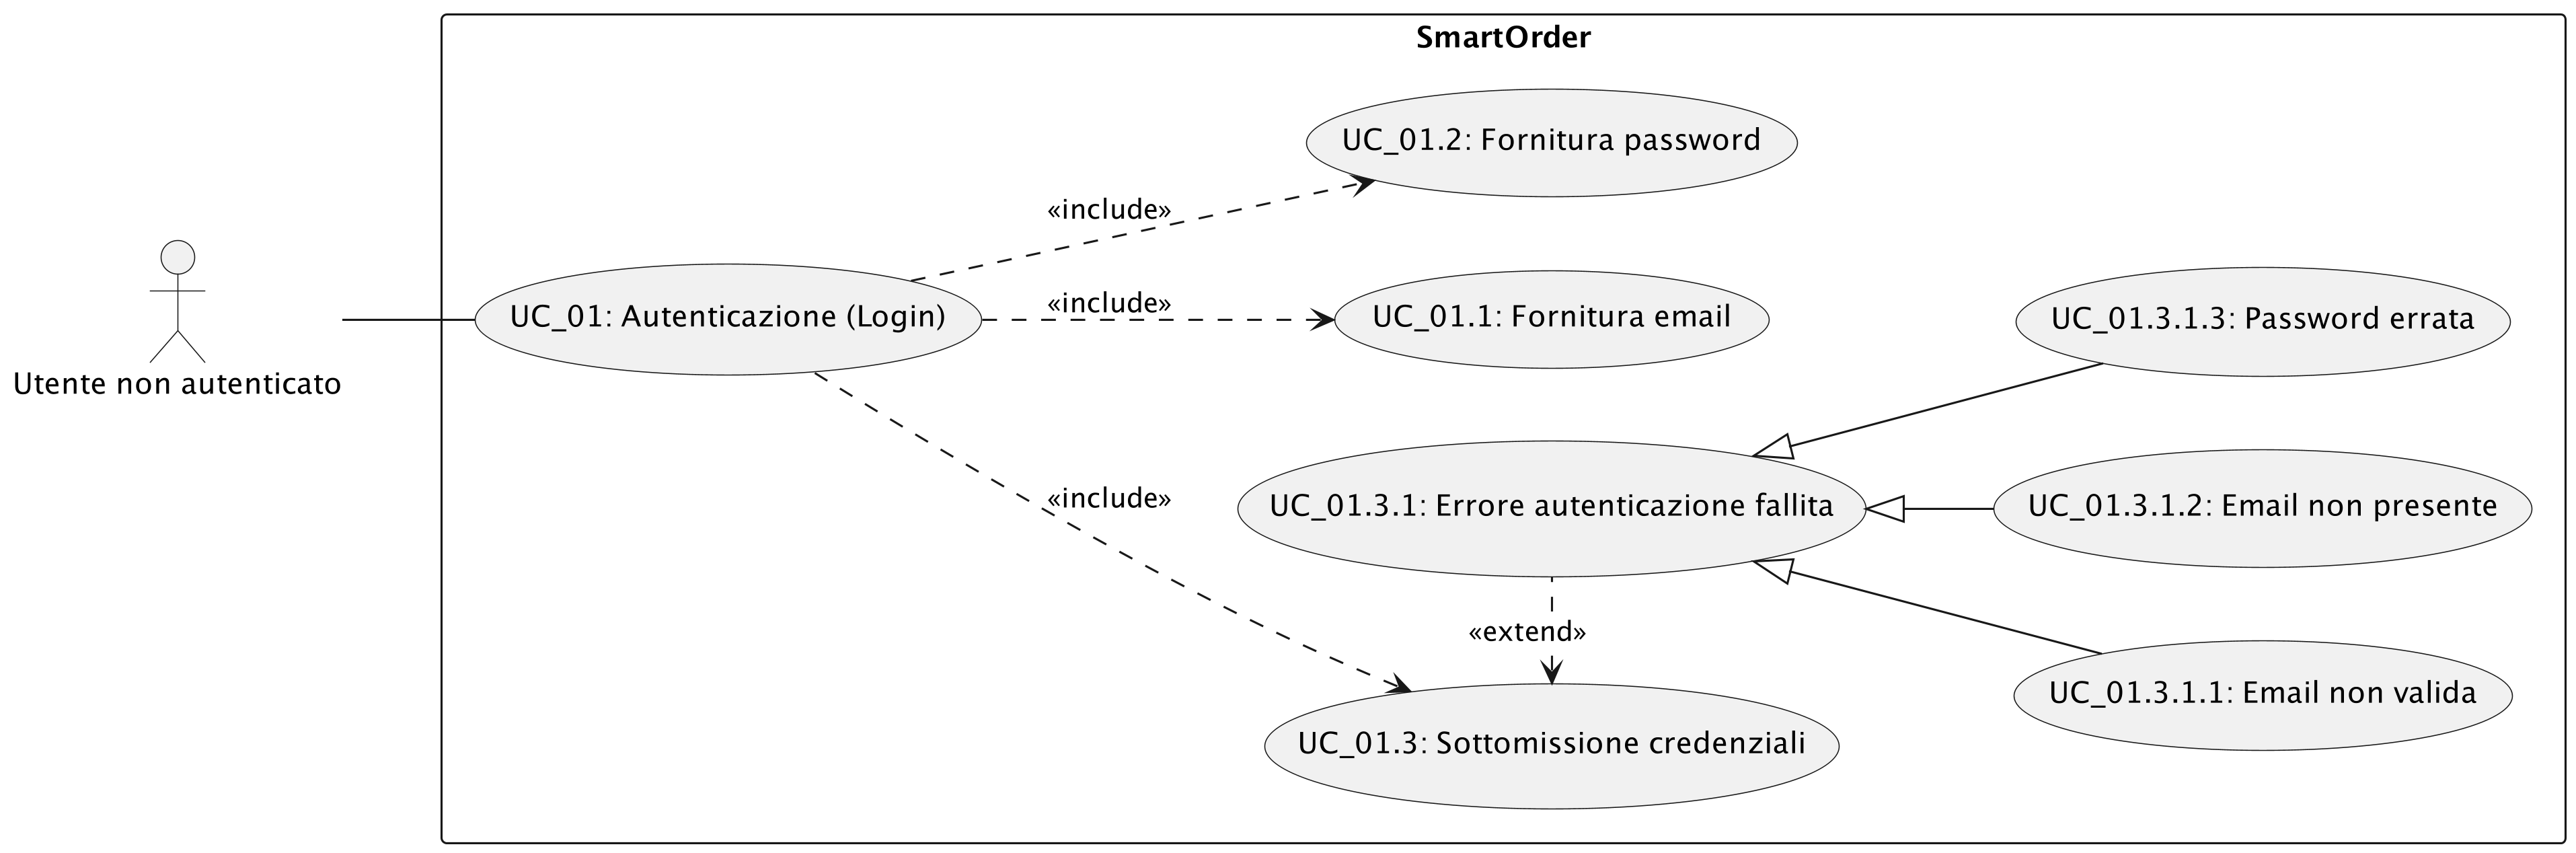
\includegraphics[width=0.8\textwidth]{uc-1.png}
    \caption{UC\_01: Autenticazione (Login)}
\end{figure}

\begin{itemize}
    \item \textbf{Attore\textsubscript{\textsc{g}} Principale}: Utente non autenticato
    \item \textbf{User Story}: Come Utente non autenticato, voglio accedere al sistema fornendo le mie credenziali, affinché io possa utilizzare la piattaforma nel mio ruolo specifico.
    \item \textbf{Scenario Principale}: 
    \begin{enumerate}
        \item Fornitura dell'email $\rightarrow$ Vedi \hyperref[uc_01.1]{UC\_01.1}
        \item Fornitura della password $\rightarrow$ Vedi \hyperref[uc_01.2]{UC\_01.2}
        \item Sottomissione delle credenziali $\rightarrow$ Vedi \hyperref[uc_01.3]{UC\_01.3}
    \end{enumerate}
    \item \textbf{Precondizioni}:
    \begin{itemize}
        \item Il sistema è operativo.
        \item L'Utente non è autenticato ed è in fase di identificazione.
    \end{itemize}
    \item \textbf{Postcondizioni}:
    \begin{itemize}
        \item L'Utente viene autenticato e il sistema gli concede l'accesso all'area operativa corrispondente al proprio ruolo (Cliente o Operatore).
    \end{itemize}
    \item \textbf{Inclusioni}:
    \begin{itemize}
        \item \hyperref[uc_01.1]{UC\_01.1}, \hyperref[uc_01.2]{UC\_01.2}, \hyperref[uc_01.3]{UC\_01.3}
    \end{itemize}
    \item \textbf{Trigger}: L'Utente manifesta l'intenzione di accedere a una risorsa privata del sistema.
\end{itemize}

\subsubsection{UC\_01.1: Fornitura email}
\label{uc_01.1}
\begin{itemize}
    \item \textbf{Attore Principale}: Utente non autenticato
    \item \textbf{Scenario Principale}: L'Utente immette a sistema l'indirizzo email associato al proprio account.
    \item \textbf{Precondizioni}: Il sistema è in attesa di ricevere le credenziali.
    \item \textbf{Postcondizioni}: Il dato relativo all'email viene acquisito dal modulo d'accesso.
\end{itemize}

\subsubsection{UC\_01.2: Fornitura password}
\label{uc_01.2}
\begin{itemize}
    \item \textbf{Attore Principale}: Utente non autenticato
    \item \textbf{Scenario Principale}: L'Utente immette la propria password a sistema (con input visivamente offuscato per sicurezza).
    \item \textbf{Postcondizioni}: Il dato relativo alla password viene acquisito in modo protetto.
\end{itemize}

\subsubsection{UC\_01.3: Sottomissione credenziali}
\label{uc_01.3}
\begin{itemize}
    \item \textbf{Attore Principale}: Utente non autenticato
    \item \textbf{Scenario Principale}:
    \begin{enumerate}
        \item L'Utente conferma l'intenzione di procedere con l'autenticazione.
        \item Il sistema verifica la correttezza della combinazione dei dati incrociandola con il database locale.
    \end{enumerate}
    \item \textbf{Precondizioni}: L'Utente ha fornito i dati logici di identificazione.
    \item \textbf{Postcondizioni}: Il sistema riconosce l'Utente, istanzia la sessione e ne autorizza l'ingresso nell'area riservata.
    \item \textbf{Estensioni}:
    \begin{itemize}
        \item Il sistema rileva un'anomalia nei dati forniti $\rightarrow$ Vedi \hyperref[uc_01.3.1]{UC\_01.3.1}
    \end{itemize}
    \item \textbf{Trigger}: L'Utente comanda l'esecuzione formale del login.
\end{itemize}

\paragraph{UC\_01.3.1: Errore autenticazione fallita}\mbox{}\\[0.1cm]
\label{uc_01.3.1}
\begin{itemize}
    \item \textbf{Attore Principale}: Utente non autenticato
    \item \textbf{Scenario Principale}: La procedura di validazione backend fallisce a causa di parametri non idonei.
    \item \textbf{Postcondizioni}: Il sistema nega l'accesso, mantiene l'Utente nello stato di non autenticato e notifica esplicitamente la motivazione dell'errore.
    \item \textbf{Specializzazioni}:
    \begin{itemize}
        \item Email non valida :L'input non rispetta le regole semantiche standard.
        \item Email non presente nel sistema :Nessuna corrispondenza anagrafica nel DB locale.
        \item Password errata :L'hash crittografico fornito non coincide con quello salvato.
    \end{itemize}
\end{itemize}

% -------------------------------------------------------------------

\subsection{UC\_02: Recupero password dimenticata}
\label{uc_02}

\begin{figure}[H]
    \centering 
    
\includegraphics[width=0.8\textwidth]{uc-2.png}
    \caption{UC\_02: Recupero password dimenticata}
\end{figure}

\begin{itemize}
    \item \textbf{Attore Principale}: Utente non autenticato
    \item \textbf{User Story}: Come Utente non autenticato, voglio richiedere un link di ripristino per la mia password in caso di smarrimento.
    \item \textbf{Scenario Principale}:
    \begin{enumerate}
        \item L'Utente richiede l'accesso alla procedura di recupero.
        \item Fornitura dell'email di contatto $\rightarrow$ Vedi \hyperref[uc_02.1]{UC\_02.1}
        \item Sottomissione della richiesta di recupero $\rightarrow$ Vedi \hyperref[uc_02.2]{UC\_02.2}
    \end{enumerate}
    \item \textbf{Precondizioni}: L'Utente non è autenticato.
    \item \textbf{Postcondizioni}: Il sistema elabora la richiesta e predispone l'invio della comunicazione di ripristino.
    \item \textbf{Inclusioni}: \hyperref[uc_02.1]{UC\_02.1}, \hyperref[uc_02.2]{UC\_02.2}
    \item \textbf{Trigger}: L'Utente manifesta la necessità di resettare le proprie credenziali tramite l'apposito comando.
\end{itemize}

\subsubsection{UC\_02.1: Fornitura email di contatto}
\label{uc_02.1}
\begin{itemize}
    \item \textbf{Attore Principale}: Utente non autenticato
    \item \textbf{Scenario Principale}: L'Utente immette a sistema il proprio indirizzo di posta elettronica all'interno del modulo dedicato.
\end{itemize}

\subsubsection{UC\_02.2: Sottomissione richiesta di recupero}
\label{uc_02.2}
\begin{itemize}
    \item \textbf{Attore Principale}: Utente non autenticato
    \item \textbf{Scenario Principale}:
    \begin{enumerate}
        \item L'Utente conferma la volontà di inoltrare la richiesta di recupero.
        \item Il sistema convalida la presenza del contatto nel DB locale e innesca la generazione della mail.
    \end{enumerate}
    \item \textbf{Postcondizioni}: Il sistema accoda il messaggio logico per l'invio e notifica all'Utente la presa in carico dell'operazione.
    \item \textbf{Estensioni}:
    \begin{itemize}
        \item Il contatto fornito è sintatticamente invalido oppure inesistente a sistema $\rightarrow$ L'invio viene inibito preventivamente e l'anomalia viene notificata a schermo.
    \end{itemize}
\end{itemize}

% -------------------------------------------------------------------

\subsection{UC\_03: Terminazione Sessione (Logout)}
\label{uc_03}

\begin{figure}[H]
    \centering 
    
\includegraphics[width=0.8\textwidth]{uc-3.png}
    \caption{UC\_03: Terminazione Sessione (Logout)}
\end{figure}

\begin{itemize}
    \item \textbf{Attore Principale}: Utente
    \item \textbf{User Story}: Come Utente loggato, voglio poter terminare la mia sessione in totale sicurezza per prevenire accessi non autorizzati.
    \item \textbf{Scenario Principale}: L'Utente comanda l'uscita esplicita dal sistema interagendo con il controllo dedicato.
    \item \textbf{Precondizioni}: L'Utente possiede una sessione di autenticazione attiva.
    \item \textbf{Postcondizioni}: Il sistema invalida e distrugge la sessione corrente lato server, revocando le autorizzazioni dell'Utente e riportandolo alla schermata pubblica di login.
\end{itemize}

% -------------------------------------------------------------------

\subsection{UC\_04: Consultazione Area Personale}
\label{uc_04}

\begin{figure}[H]
    \centering 
    
\includegraphics[width=0.8\textwidth]{uc-4.png}
    \caption{UC\_04: Consultazione Area Personale}
\end{figure}

\begin{itemize}
    \item \textbf{Attore Principale}: Utente
    \item \textbf{User Story}: Come Utente loggato, voglio accedere al riepilogo del mio profilo per verificare i dati anagrafici a me associati.
    \item \textbf{Scenario Principale}:
    \begin{enumerate}
        \item L'Utente richiede l'accesso alla rotta dedicata al profilo.
        \item \textit{[Solo se l'Utente possiede il ruolo "Cliente"]} Il sistema espone le informazioni anagrafiche aziendali $\rightarrow$ \hyperref[uc_00.2]{UC\_00.2}
        \item Esposizione dell'Indirizzo Email $\rightarrow$ Vedi \hyperref[uc_04.1]{UC\_04.1}
        \item Esposizione opzione di modifica credenziali $\rightarrow$ Vedi \hyperref[uc_04.2]{UC\_04.2}
    \end{enumerate}
    \item \textbf{Precondizioni}: L'Utente è riconosciuto dal sistema tramite sessione attiva.
    \item \textbf{Postcondizioni}: Il sistema rende disponibili i dati in base ai permessi di ruolo.
    \item \textbf{Inclusioni}: \hyperref[uc_00.2]{UC\_00.2}, \hyperref[uc_04.1]{UC\_04.1}, \hyperref[uc_04.2]{UC\_04.2}
    \item \textbf{Trigger}: Navigazione volontaria verso la sezione del profilo personale.
\end{itemize}

\subsubsection{UC\_04.1: Esposizione Indirizzo Email (Sola lettura)}
\label{uc_04.1}
\begin{itemize}
    \item \textbf{Attore Principale}: Utente
    \item \textbf{Scenario Principale}: Il sistema preleva dal DB locale e restituisce a schermo l'indirizzo email identificativo dell'Utente in modalità immutabile.
\end{itemize}

\subsubsection{UC\_04.2: Esposizione opzione di modifica credenziali}
\label{uc_04.2}
\begin{itemize}
    \item \textbf{Attore Principale}: Utente
    \item \textbf{Scenario Principale}: Il sistema presenta all'Utente l'accesso logico (es. pulsante o link) per avviare la mutazione della chiave di sicurezza, ponendosi in ascolto per l'attivazione del caso d'uso \hyperref[uc_05]{UC\_05}.
\end{itemize}

% -------------------------------------------------------------------

\subsection{UC\_05: Cambio Password}
\label{uc_05}

\begin{figure}[H]
    \centering 
    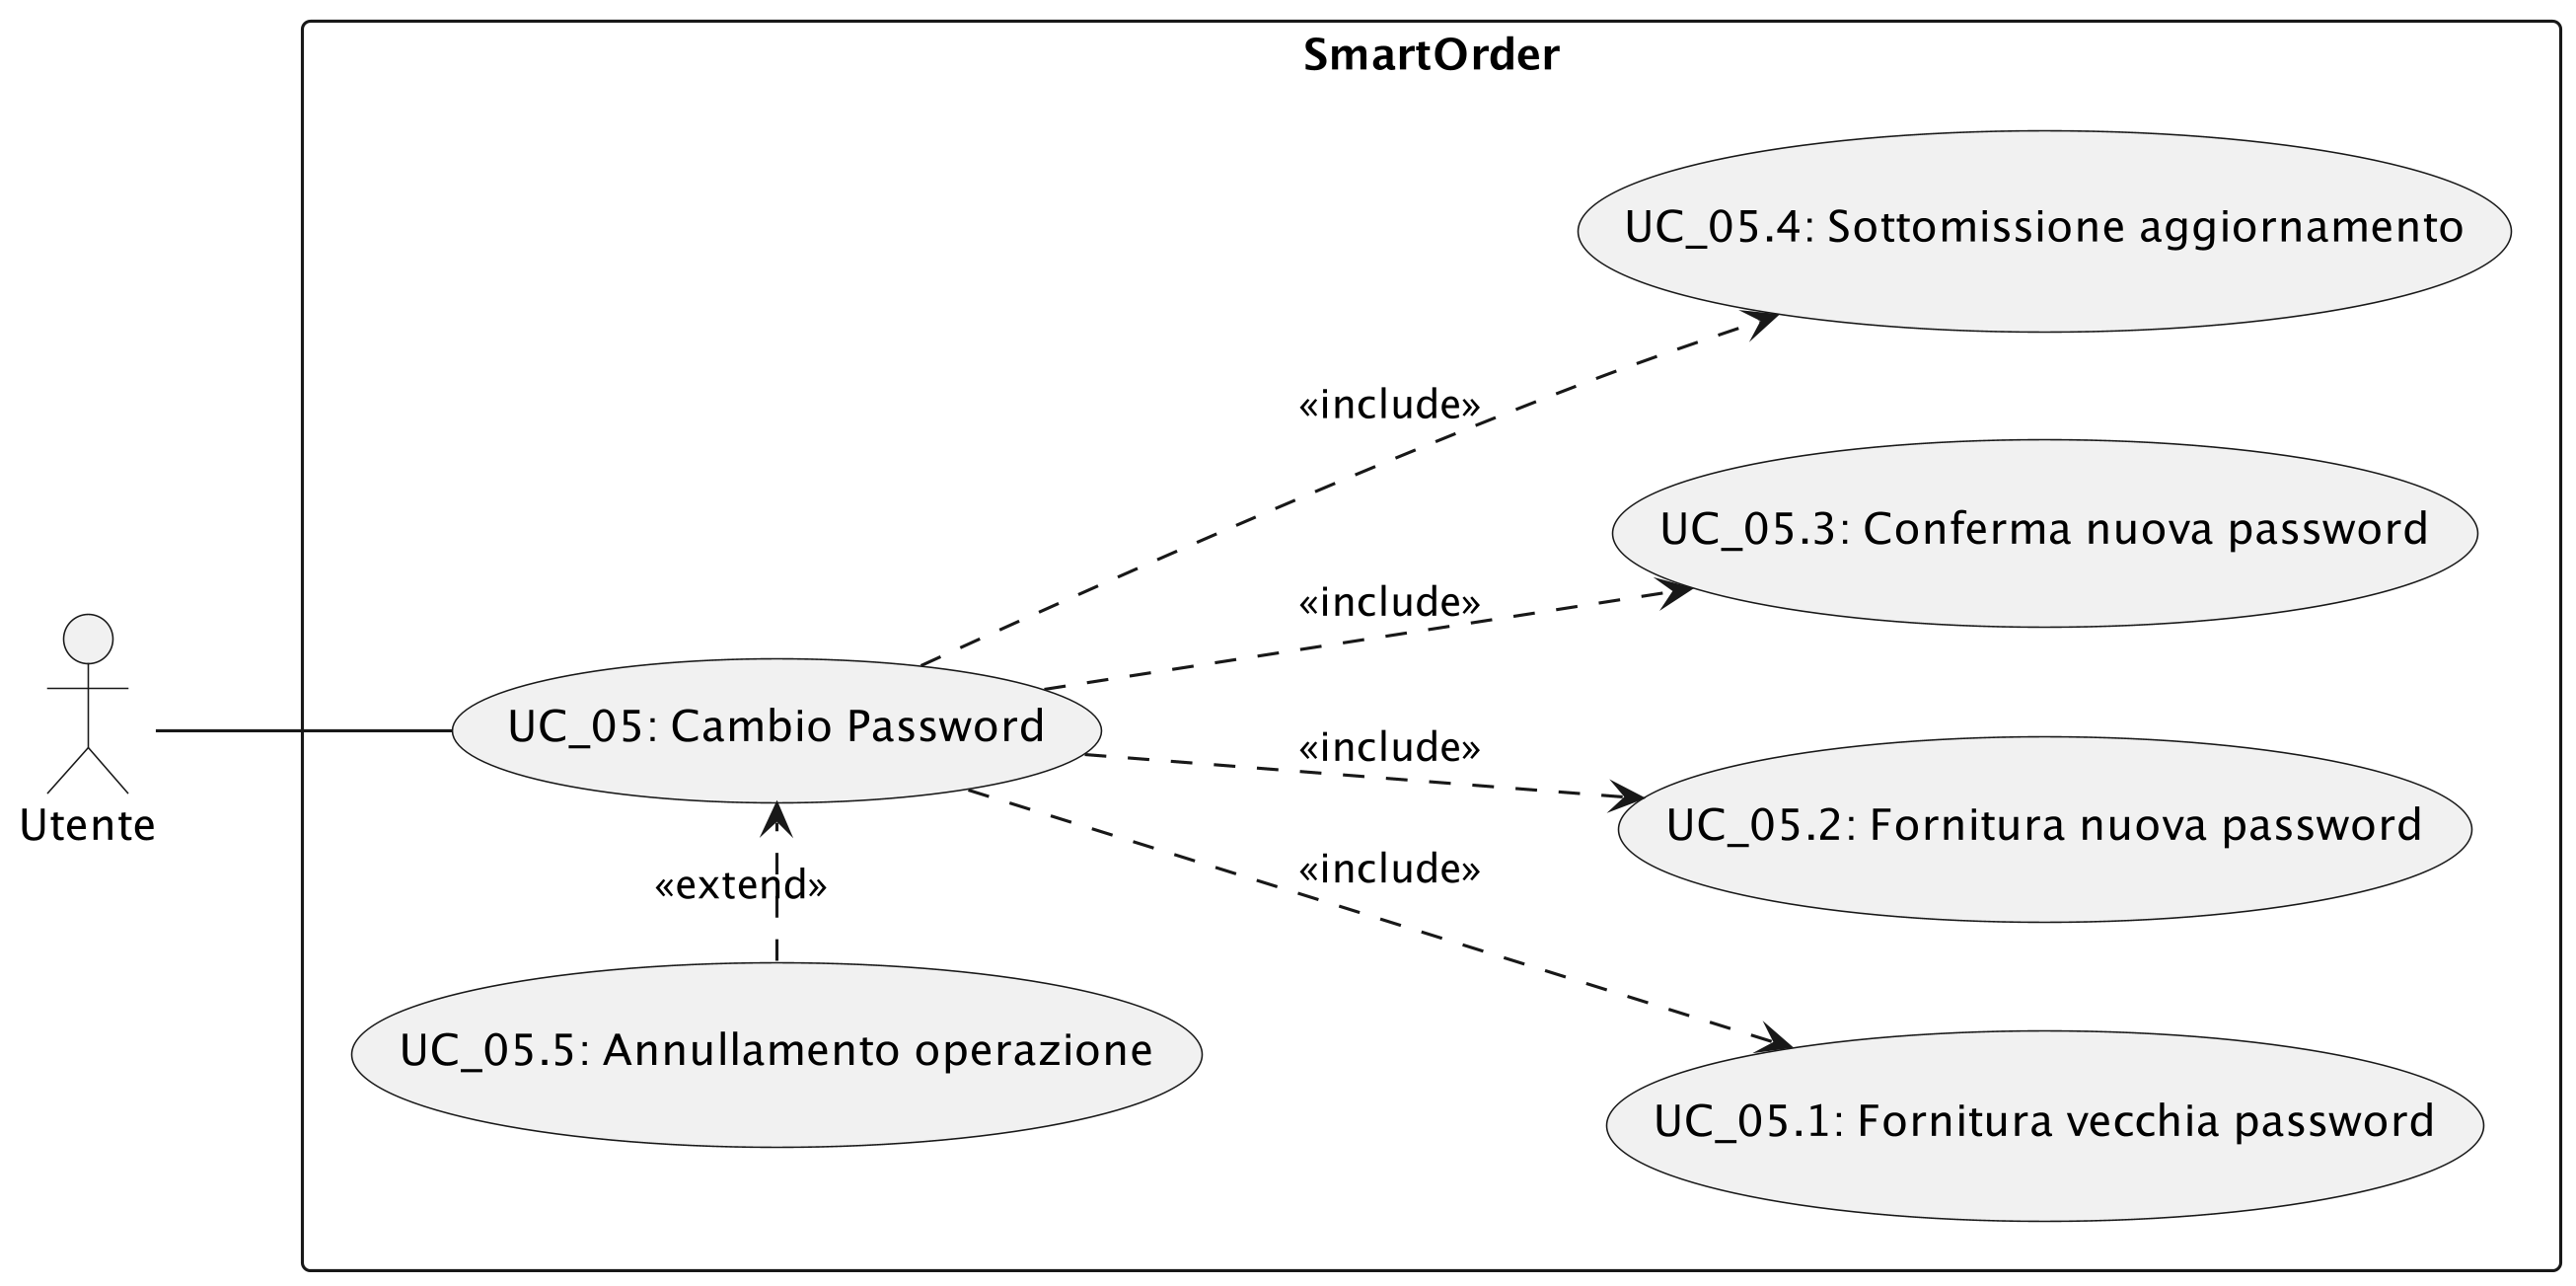
\includegraphics[width=0.8\textwidth]{uc-5.png}
    \caption{UC\_05: Cambio Password}
\end{figure}

\begin{itemize}
    \item \textbf{Attore Principale}: Utente
    \item \textbf{User Story}: Come Utente loggato, voglio rimpiazzare la mia password attuale con una nuova per garantire la sicurezza del mio account.
    \item \textbf{Nota Requisito}: Funzionalità classificata come requisito desiderabile.
    \item \textbf{Scenario Principale}:
    \begin{enumerate}
        \item Fornitura vecchia password $\rightarrow$ Vedi \hyperref[uc_05.1]{UC\_05.1}
        \item Fornitura nuova password $\rightarrow$ Vedi \hyperref[uc_05.2]{UC\_05.2}
        \item Fornitura conferma nuova password $\rightarrow$ Vedi \hyperref[uc_05.3]{UC\_05.3}
        \item Sottomissione aggiornamento $\rightarrow$ Vedi \hyperref[uc_05.4]{UC\_05.4}
    \end{enumerate}
    \item \textbf{Precondizioni}: L'Utente ha richiesto esplicitamente l'avvio della procedura dalla propria Area Personale.
    \item \textbf{Postcondizioni}: La sequenza di accesso crittografica dell'Utente viene aggiornata in via definitiva nel sistema.
    \item \textbf{Inclusioni}: \hyperref[uc_05.1]{UC\_05.1}, \hyperref[uc_05.2]{UC\_05.2}, \hyperref[uc_05.3]{UC\_05.3}, \hyperref[uc_05.4]{UC\_05.4}
    \item \textbf{Estensioni}: L'Utente opta per l'annullamento volontario dismettendo la procedura $\rightarrow$ Vedi \hyperref[uc_05.5]{UC\_05.5}
\end{itemize}

\subsubsection{UC\_05.1: Fornitura vecchia password}
\label{uc_05.1}
\begin{itemize}
    \item \textbf{Attore Principale}: Utente
    \item \textbf{Scenario Principale}: L'Utente immette a sistema la sequenza di sicurezza attualmente in vigore per scopi di convalida.
    \item \textbf{Estensioni}: Il sistema rileva che la sequenza corrente fornita non combacia con l'hash a database. L'operazione viene interrotta e viene generata un'anomalia.
\end{itemize}

\subsubsection{UC\_05.2: Fornitura nuova password}
\label{uc_05.2}
\begin{itemize}
    \item \textbf{Attore Principale}: Utente
    \item \textbf{Scenario Principale}: L'Utente immette a sistema la nuova sequenza desiderata, ottemperando alle policy architetturali di robustezza.
\end{itemize}

\subsubsection{UC\_05.3: Fornitura conferma nuova password}
\label{uc_05.3}
\begin{itemize}
    \item \textbf{Attore Principale}: Utente
    \item \textbf{Scenario Principale}: L'Utente re-immette la nuova sequenza per verificarne l'esattezza digitativa.
    \item \textbf{Estensioni}: Il sistema valuta l'assenza di identità tra la stringa di nuova password e quella di conferma. L'aggiornamento viene impedito con notifica d'errore.
\end{itemize}

\subsubsection{UC\_05.4: Sottomissione aggiornamento}
\label{uc_05.4}
\begin{itemize}
    \item \textbf{Attore Principale}: Utente
    \item \textbf{Scenario Principale}: L'Utente comanda il consolidamento delle modifiche. Il sistema esegue i controlli di validità e sovrascrive l'hash crittografico.
    \item \textbf{Postcondizioni}: La procedura si chiude restituendo una conferma di avvenuta esecuzione logica.
\end{itemize}

\subsubsection{UC\_05.5: Annullamento operazione}
\label{uc_05.5}
\begin{itemize}
    \item \textbf{Attore Principale}: Utente
    \item \textbf{Scenario Principale}: L'Utente comanda l'abbandono volontario della procedura.
    \item \textbf{Postcondizioni}: L'operazione decade transitoriamente. Il sistema dismette i parametri acquisiti ripristinando il normale stato di consultazione del profilo.
\end{itemize}

% -------------------------------------------------------------------
  
\subsection{UC\_06: Richiesta di contatto supporto tecnico}
\label{uc_06}

\begin{figure}[H]
    \centering 
    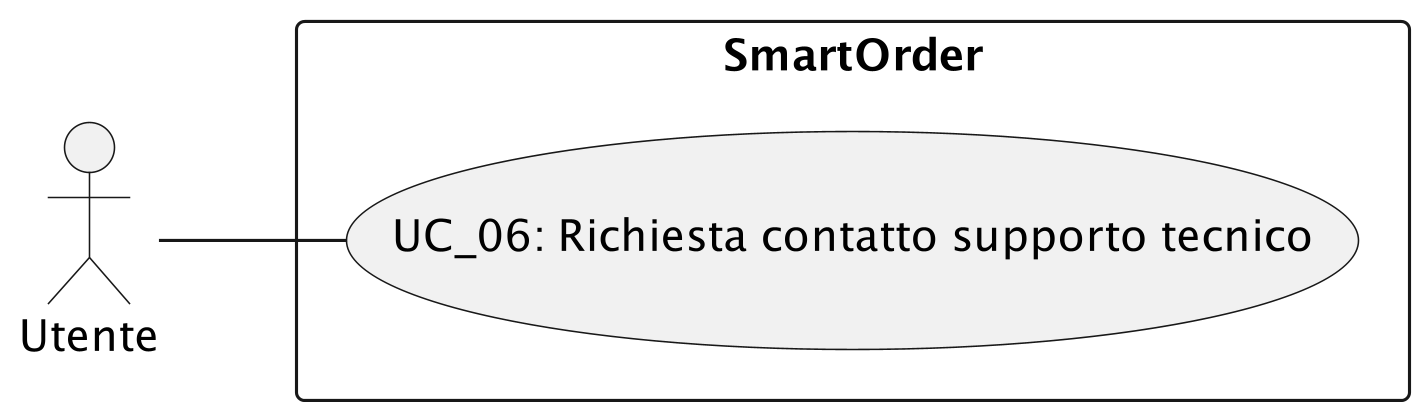
\includegraphics[width=0.8\textwidth]{uc-6.png}
    \caption{UC\_06: Richiesta di contatto supporto tecnico}
\end{figure}
 
\begin{itemize}
    \item \textbf{Attori Principali}: Utente non autenticato, Utente
    \item \textbf{User Story}: Come Utente, voglio avere un'opzione rapida per inoltrare comunicazioni amministrative tramite il mio sistema di posta elettronica nativo.
    \item \textbf{Scenario Principale}:
    \begin{enumerate}
        \item L'Utente comanda l'attivazione della funzionalità di contatto globale.
        \item Il sistema invoca il protocollo operativo standard (URI di tipo \textit{mailto:}).
        \item Il sistema operativo locale intercetta l'invocazione lanciando il software di composizione email, valorizzando automaticamente il destinatario.
    \end{enumerate}
    \item \textbf{Precondizioni}: L'Utente ha accesso alle funzionalità generali e il dispositivo locale possiede un client email configurato.
    \item \textbf{Postcondizioni}: L'azione esce dal perimetro dell'applicativo web.
    \item \textbf{Trigger}: Manifestazione della necessità di instaurare un dialogo extra-sistema.
\end{itemize}

% ==========================================
% GRUPPO B: INTERAZIONE CHAT E AI
% ==========================================

\subsection{UC\_07: Consultazione Chat (Live)}
\label{uc_07}

\begin{figure}[H]
    \centering 
    
\includegraphics[width=0.8\textwidth]{uc-7.png}
    \caption{UC\_07: Consultazione Chat}
\end{figure}

\begin{itemize}
    \item \textbf{Attore Principale}: Utente
    \item \textbf{User Story}: Come Utente, voglio poter leggere lo storico live dei messaggi all'interno della sessione corrente, affinché io possa avere chiara l'evoluzione della conversazione e le richieste già elaborate.
    \item \textbf{Scenario Principale}: 
    \begin{enumerate}
        \item L'Utente ottiene visibilità sul flusso conversazionale attivo.
        \item Il sistema espone le interazioni storicizzate, distinguendo tra messaggi in uscita dall'Utente ($\rightarrow$ Vedi \hyperref[uc_07.1]{UC\_07.1}) e risposte in ingresso dal sistema ($\rightarrow$ Vedi \hyperref[uc_07.2]{UC\_07.2}).
    \end{enumerate}
    \item \textbf{Precondizioni}: L'Utente si trova nell'area operativa principale ed è agganciato a una sessione di chat attiva.
    \item \textbf{Postcondizioni}: La vista si aggiorna asincronamente in tempo reale alla ricezione o all'invio di nuovi payload.
    \item \textbf{Inclusioni}: \hyperref[uc_07.1]{UC\_07.1}, \hyperref[uc_07.2]{UC\_07.2}
    \item \textbf{Trigger}: Caricamento dell'interfaccia o ricezione di un nuovo pacchetto testuale.
\end{itemize}

\subsubsection{UC\_07.1: Esposizione log input Utente}
\label{uc_07.1}
\begin{itemize}
    \item \textbf{Attore Principale}: Utente
    \item \textbf{Scenario Principale}: Il sistema formatta e renderizza a schermo gli input pregressi (trascrizioni testuali, metadati audio o documentali) originati dal terminale dell'Utente.
    \item \textbf{Postcondizioni}: Il messaggio è visualmente associato e ancorato al mittente (es. tramite allineamento strutturale o codifica cromatica).
\end{itemize}

\subsubsection{UC\_07.2: Esposizione log risposte Sistema/AI}
\label{uc_07.2}
\begin{itemize}
    \item \textbf{Attore Principale}: Utente
    \item \textbf{Scenario Principale}: Il sistema formatta e renderizza a schermo gli output testuali o le schede prodotto generate in risposta dal modello LLM (o inoltrati dall'Operatore in fase di subentro).
    \item \textbf{Postcondizioni}: La risposta è identificabile inequivocabilmente come reazione della piattaforma.
\end{itemize}

% -------------------------------------------------------------------

\subsection{UC\_08: Sottomissione Input Multimodale}
\label{uc_08}

\begin{figure}[H]
    \centering 
    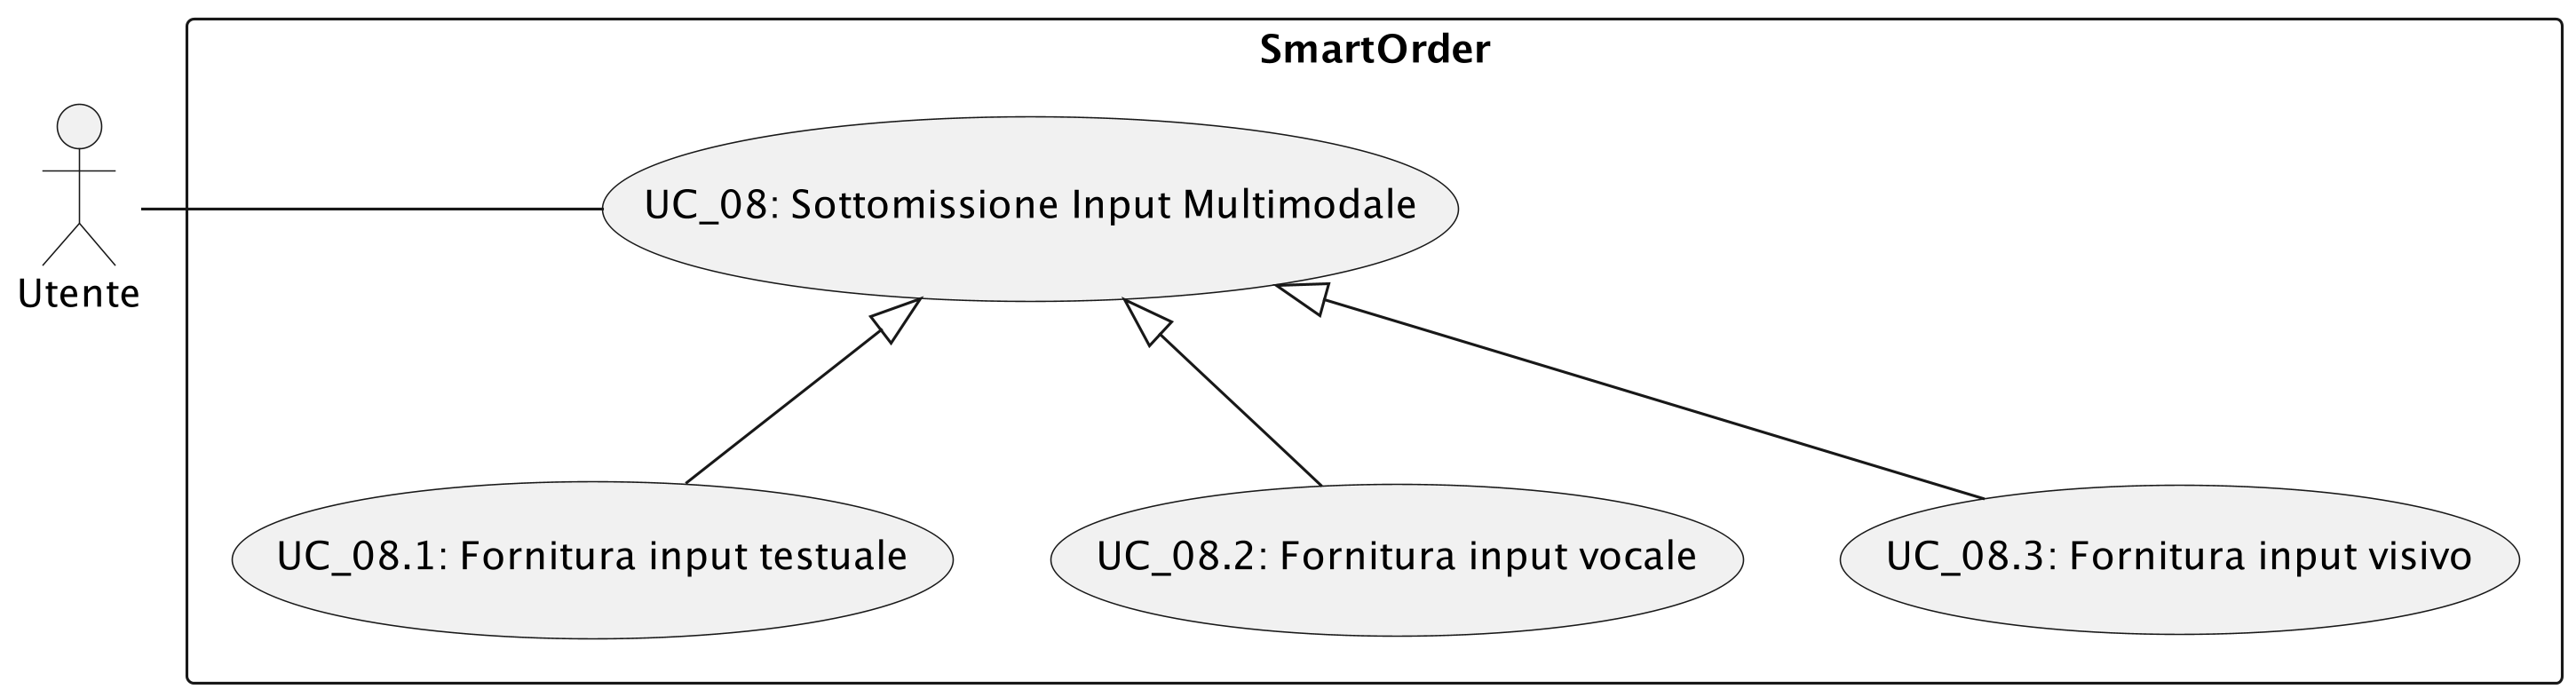
\includegraphics[width=0.8\textwidth]{uc-8.png}
    \caption{UC\_08: Sottomissione Input Multimodale}
\end{figure}

\begin{itemize}
    \item \textbf{Attore Principale}: Utente
    \item \textbf{User Story}: Come Utente, voglio poter inviare richieste al sistema utilizzando diverse modalità (testo, voce, immagini) per formulare un comando nel modo più efficiente possibile a seconda del mio contesto.
    \item \textbf{Scenario Principale}:
    \begin{enumerate}
        \item L'Utente determina la modalità di inserimento dati preferita interagendo con l'interfaccia.
        \item Immissione tramite canale testuale $\rightarrow$ Vedi \hyperref[uc_08.1]{UC\_08.1}
        \item Immissione tramite canale vocale $\rightarrow$ Vedi \hyperref[uc_08.2]{UC\_08.2}
        \item Immissione tramite acquisizione visiva $\rightarrow$ Vedi \hyperref[uc_08.3]{UC\_08.3}
    \end{enumerate}
    \item \textbf{Precondizioni}:
    \begin{itemize}
        \item L'Utente ha accesso ai controlli di interazione della conversazione attiva.
    \end{itemize}
    \item \textbf{Postcondizioni}:
    \begin{itemize}
        \item Il payload (testuale o multimediale) viene confezionato dal frontend e trasmesso al backend locale per il processamento o l'inoltro all'Intelligenza Artificiale. Il sistema si pone in attesa asincrona della risposta.
    \end{itemize}
    \item \textbf{Specializzazioni}:
    \begin{itemize}
        \item \hyperref[uc_08.1]{UC\_08.1}, \hyperref[uc_08.2]{UC\_08.2}, \hyperref[uc_08.3]{UC\_08.3}
    \end{itemize}
    \item \textbf{Trigger}: L'Utente avvia la composizione di un nuovo messaggio.
\end{itemize}

\subsubsection{UC\_08.1: Fornitura di input testuale}
\label{uc_08.1}
\begin{itemize}
    \item \textbf{Attore Principale}: Utente
    \item \textbf{Scenario Principale}: L'Utente formula il proprio messaggio digitandolo nel modulo dedicato e ne comanda l'invio logico.
    \item \textbf{Postcondizioni}: La stringa testuale viene validata e immessa nel flusso dati verso l'analizzatore semantico.
    \item \textbf{Estensioni}:
    \begin{itemize}
        \item Se l'input testuale eccede i limiti dimensionali architetturali $\rightarrow$ Il sistema interrompe l'invio preventivamente, mantiene il testo a disposizione per correzioni e notifica l'impossibilità di procedere a causa dell'eccessiva lunghezza.
    \end{itemize}
\end{itemize}

\subsubsection{UC\_08.2: Fornitura di input vocale}
\label{uc_08.2}
\begin{itemize}
    \item \textbf{Attore Principale}: Utente
    \item \textbf{Scenario Principale}: L'Utente avvia l'acquisizione microfonica, detta la richiesta vocalmente e arresta la registrazione comandandone la trasmissione.
    \item \textbf{Precondizioni}: Il dispositivo ospite possiede i permessi hardware di cattura audio.
    \item \textbf{Postcondizioni}: Il file audio viene trasmesso al modulo Speech-to-Text per la conversione in stringa elaborabile.
    \item \textbf{Estensioni}:
    \begin{itemize}
        \item Se il file audio eccede il peso massimo consentito (es. 10MB) $\rightarrow$ Il caricamento viene inibito con esposizione di notifica d'errore.
    \end{itemize}
\end{itemize}

\subsubsection{UC\_08.3: Fornitura di input visivo (Immagine)}
\label{uc_08.3}
\begin{itemize}
    \item \textbf{Attore Principale}: Utente
    \item \textbf{Nota Requisito}: Questa funzionalità è classificata come requisito desiderabile.
    \item \textbf{Scenario Principale}: L'Utente innesca la funzione di caricamento media e seleziona la fonte di acquisizione (fotocamera hardware, galleria locale o file system).
    \item \textbf{Precondizioni}: L'ambiente operativo supporta i moduli di elaborazione OCR (Optical Character Recognition).
    \item \textbf{Postcondizioni}: L'immagine scelta viene immessa nella pipeline per l'estrazione logica del contenuto testuale o l'identificazione prodotto.
    \item \textbf{Estensioni}:
    \begin{itemize}
        \item Se l'immagine selezionata eccede il peso massimo (es. 5MB) $\rightarrow$ L'upload viene bloccato e il sistema notifica l'impossibilità di processare il file.
    \end{itemize}
\end{itemize}

% -------------------------------------------------------------------

\subsection{UC\_09: Classificazione e Feedback Risposta AI}
\label{uc_09}

\begin{figure}[H]
    \centering 
    
\includegraphics[width=0.8\textwidth]{uc-9.png}
    \caption{UC\_09: Classificazione e Feedback Risposta AI}
\end{figure}

\begin{itemize}
    \item \textbf{Attore Principale}: Cliente
    \item \textbf{User Story}: Come Cliente, voglio poter giudicare l'accuratezza semantica delle risposte del sistema per contribuire al perfezionamento dell'Intelligenza Artificiale aziendale.
    \item \textbf{Scenario Principale}:
    \begin{enumerate}
        \item Il Cliente valuta intellettualmente l'output generato dall'LLM.
        \item Sottomissione di giudizio positivo $\rightarrow$ Vedi \hyperref[uc_09.1]{UC\_09.1}
        \item Sottomissione di giudizio negativo e segnalazione anomalia $\rightarrow$ Vedi \hyperref[uc_09.2]{UC\_09.2}
    \end{enumerate}
    \item \textbf{Precondizioni}:
    \begin{itemize}
        \item Il sistema ha esposto almeno un output generato dal modello linguistico e i controlli di valutazione sono abilitati.
    \end{itemize}
    \item \textbf{Postcondizioni}:
    \begin{itemize}
        \item Il feedback viene registrato nel database locale e relazionato all'identificativo univoco della transazione AI (Log).
    \end{itemize}
    \item \textbf{Specializzazioni}:
    \begin{itemize}
        \item \hyperref[uc_09.1]{UC\_09.1}, \hyperref[uc_09.2]{UC\_09.2}
    \end{itemize}
    \item \textbf{Trigger}: Il Cliente matura un'opinione circa la congruità dell'output ricevuto.
\end{itemize}

\subsubsection{UC\_09.1: Sottomissione di valutazione positiva}
\label{uc_09.1}
\begin{itemize}
    \item \textbf{Attore Principale}: Cliente
    \item \textbf{Scenario Principale}: Il Cliente comanda l'assegnazione di un feedback logico positivo. Il sistema riceve l'impulso e lo archivia silenziamente.
    \item \textbf{Postcondizioni}: L'interfaccia inibisce valutazioni duplicate sul medesimo output.
\end{itemize}

\subsubsection{UC\_09.2: Sottomissione di valutazione negativa}
\label{uc_09.2}
\begin{itemize}
    \item \textbf{Attore Principale}: Cliente
    \item \textbf{Scenario Principale}:
    \begin{enumerate}
        \item Il Cliente manifesta l'intento di classificare la risposta come errata, causando l'esposizione di un modulo dedicato.
        \item Il Cliente seleziona obbligatoriamente i tag contestuali che definiscono la natura dell'errore (es. Errore semantico, Errore quantità).
        \item Il Cliente immette del testo libero opzionale per fornire note integrative.
        \item Il Cliente comanda il consolidamento e l'invio della segnalazione.
    \end{enumerate}
    \item \textbf{Postcondizioni}: Il sistema aggrega i parametri in un payload strutturato e genera un record d'errore (Stato "Da gestire") destinato all'ispezione nel backoffice.
    \item \textbf{Estensioni}:
    \begin{itemize}
        \item Abbandono volontario $\rightarrow$ Il Cliente comanda l'interruzione della stesura. Il modulo si chiude e i dati temporanei decadono.
    \end{itemize}
\end{itemize}

% -------------------------------------------------------------------

\subsection{UC\_10: Azzeramento del Contesto (Reset Sessione)}
\label{uc_10}

\begin{figure}[H]
    \centering 
    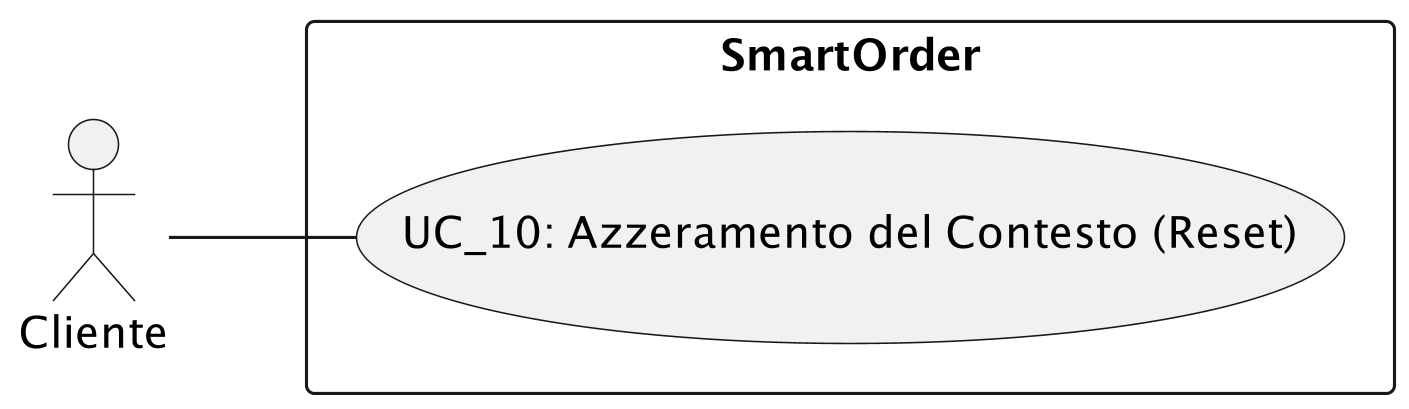
\includegraphics[width=0.8\textwidth]{uc-10.png}
    \caption{UC\_10: Azzeramento del Contesto (Reset Sessione)}
\end{figure}

\begin{itemize}
    \item \textbf{Attore Principale}: Cliente
    \item \textbf{User Story}: Come Cliente, voglio poter ripulire completamente la memoria dell'Intelligenza Artificiale per evitare interferenze tra il mio prossimo ordine e le richieste passate.
    \item \textbf{Scenario Principale}:
    \begin{enumerate}
        \item Il Cliente comanda l'instaurazione di una nuova sessione operativa tramite l'apposito controllo.
        \item Il sistema recepisce l'input ed esegue le procedure di bonifica logica lato server.
    \end{enumerate}
    \item \textbf{Precondizioni}:
    \begin{itemize}
        \item Non vi sono richieste di supporto tecnico (Ticket) pendenti o in lavorazione per la sessione attuale.
    \end{itemize}
    \item \textbf{Postcondizioni}:
    \begin{itemize}
        \item Il sistema rigetta il tracciato conversazionale precedente, svuota il carrello in memoria e associa il client a un nuovo Session ID vergine.
    \end{itemize}
    \item \textbf{Trigger}: Il Cliente necessita di un cambio radicale di contesto d'acquisto o desidera abortire la composizione in atto.
\end{itemize}

% ==========================================
% GRUPPO C: GESTIONE CARRELLO E RICERCA
% ==========================================

\subsection{UC\_11: Ricerca Manuale dei Prodotti}
\label{uc_11}

\begin{figure}[H]
    \centering 
    
\includegraphics[width=0.8\textwidth]{uc-11.png}
    \caption{UC\_11: Ricerca Manuale dei Prodotti}
\end{figure}

\begin{itemize}
    \item \textbf{Attore Principale}: Utente
    \item \textbf{User Story}: Come Utente, voglio poter cercare manualmente un prodotto specifico all'interno dell'assortimento tramite una barra di ricerca, affinché io possa individuarlo senza dover impiegare l'AI.
    \item \textbf{Scenario Principale}: 
    \begin{enumerate}
        \item Inserimento del testo di ricerca $\rightarrow$ Vedi \hyperref[uc_11.1]{UC\_11.1}
        \item Visualizzazione dinamica dei risultati filtrati $\rightarrow$ Vedi \hyperref[uc_11.2]{UC\_11.2}
    \end{enumerate}
    \item \textbf{Precondizioni}:
    \begin{itemize}
        \item L'interfaccia utente mostra la sezione dedicata al Carrello, includendo il modulo di ricerca abilitato.
    \end{itemize}
    \item \textbf{Postcondizioni}:
    \begin{itemize}
        \item Il sistema processa la stringa inserita ed esegue una query al database locale per estrarre il subset di prodotti pertinenti.
    \end{itemize}
    \item \textbf{Inclusioni}:
    \begin{itemize}
        \item \hyperref[uc_11.1]{UC\_11.1}, \hyperref[uc_11.2]{UC\_11.2}
    \end{itemize}
    \item \textbf{Trigger}: Attivazione del modulo di ricerca manuale per l'immissione della query.
\end{itemize}

\subsubsection{UC\_11.1: Inserimento testo di ricerca}
\label{uc_11.1}
\begin{itemize}
    \item \textbf{Attore Principale}: Utente
    \item \textbf{Scenario Principale}: L'Utente immette una sequenza di caratteri alfanumerici all'interno del campo di testo, innescando l'intercettazione dell'input (Live Search).
\end{itemize}

\subsubsection{UC\_11.2: Visualizzazione dinamica dei risultati}
\label{uc_11.2}
\begin{itemize}
    \item \textbf{Attore Principale}: Utente
    \item \textbf{Scenario Principale}:
    \begin{enumerate}
        \item Il sistema genera e mostra una lista contestuale di risultati validi.
        \item Per ogni referenza trovata, il sistema ne espone i metadati anagrafici logistici $\rightarrow$ Include: \hyperref[uc_00.1]{UC\_00.1}
    \end{enumerate}
    \item \textbf{Precondizioni}: Il sistema ha filtrato i risultati escludendo i prodotti dismessi e applicando le regole di visibilità catalogo associate all'anagrafica aziendale in esame (es. tabella \texttt{asscli}).
    \item \textbf{Postcondizioni}: L'elenco è visibile a schermo e le righe dei prodotti sono interattive per la selezione in fase d'aggiunta.
    \item \textbf{Inclusioni}: \hyperref[uc_00.1]{UC\_00.1}
\end{itemize}

% -------------------------------------------------------------------

\subsection{UC\_12: Aggiunta Manuale da Ricerca}
\label{uc_12}

\begin{figure}[H]
    \centering 
    
\includegraphics[width=0.8\textwidth]{uc-12.png}
    \caption{UC\_12: Aggiunta Manuale da Ricerca}
\end{figure}

\begin{itemize}
    \item \textbf{Attore Principale}: Utente
    \item \textbf{User Story}: Come Utente, una volta individuato l'articolo d'interesse, voglio poter definire con precisione quante unità acquistarne tramite un'interfaccia dedicata, prima di confermarne l'inserimento.
    \item \textbf{Scenario Principale}: 
    \begin{enumerate}
        \item L'Utente seleziona uno specifico prodotto tra i risultati proposti (\hyperref[uc_11.2]{UC\_11.2}) attivando un'interfaccia temporanea.
        \item Variazione logica incrementale/decrementale quantità oppure immissione numerica diretta.
        \item Conferma dell'inserimento definitivo tramite apposito controllo.
    \end{enumerate}
    \item \textbf{Postcondizioni}:
    \begin{itemize}
        \item L'articolo viene registrato nel database di sessione (proprio o in delega per l'Operatore), aggiunto alla lista del carrello con la quantità impostata e l'interfaccia temporanea viene destituita.
    \end{itemize}
    \item \textbf{Estensioni}:
    \begin{itemize}
        \item Violazione vincoli numerici $\rightarrow$ Se l'Utente tenta l'inserimento di valori nulli, negativi o fuori dal limite logico, il sistema impedisce l'azione e attua una correzione forzata verso il limite accettabile più vicino.
        \item Annullamento $\rightarrow$ L'Utente comanda la dismissione dell'interfaccia. Nessuna alterazione viene apportata al carrello.
    \end{itemize}
    \item \textbf{Trigger}: Selezione esplicita di una referenza dall'elenco ricerca.
\end{itemize}

% -------------------------------------------------------------------

\subsection{UC\_13: Visualizzazione e Gestione Carrello}
\label{uc_13}

\begin{figure}[H]
    \centering 
    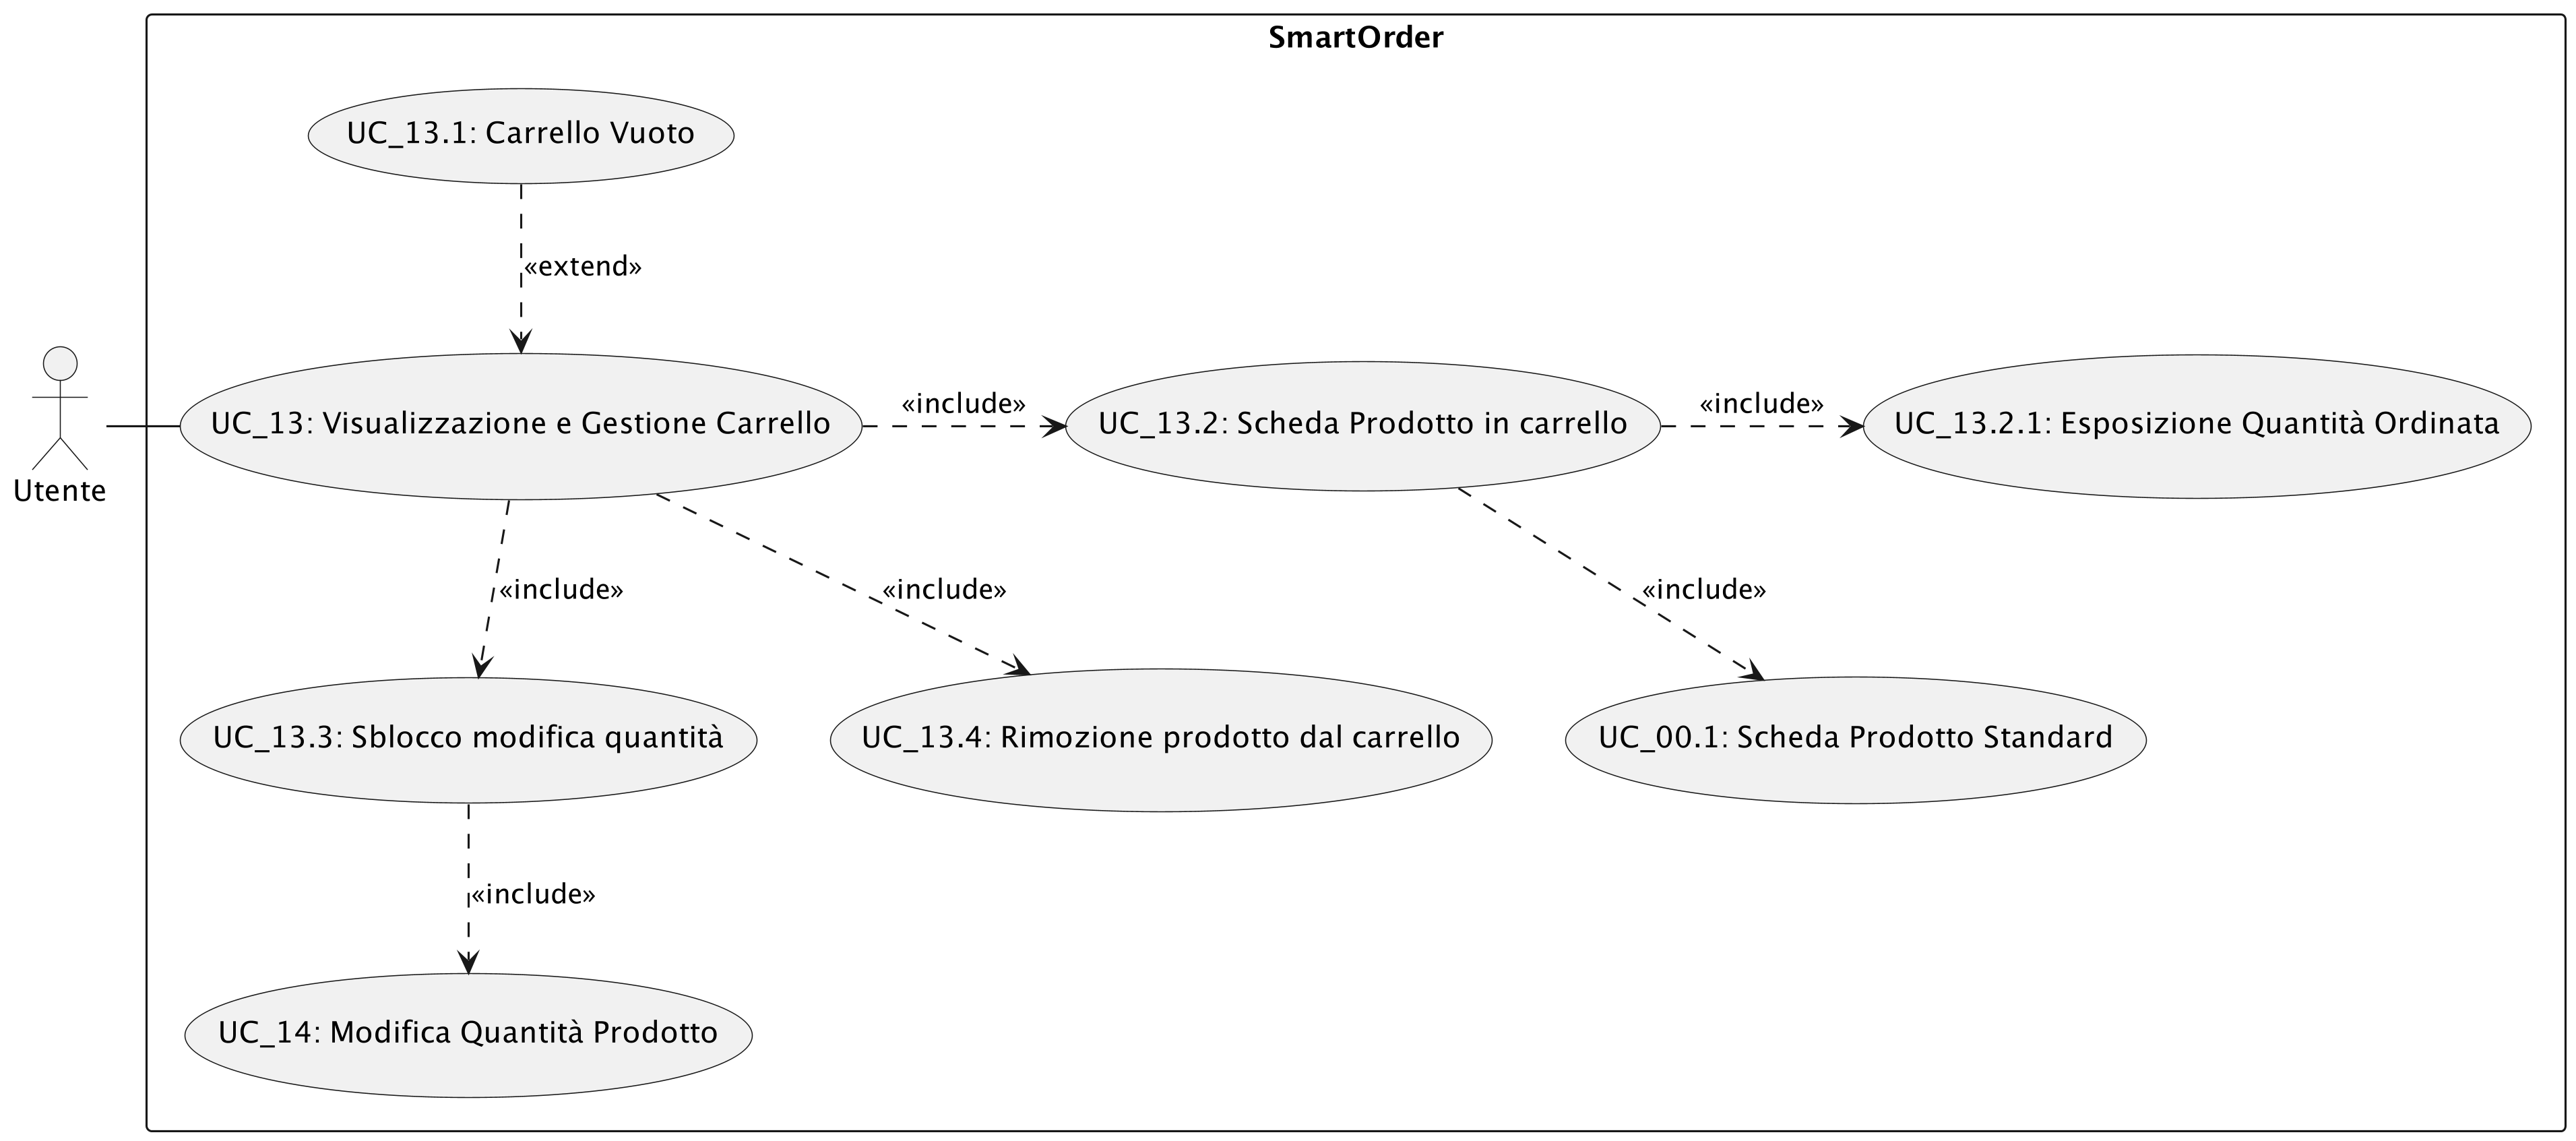
\includegraphics[width=0.9\textwidth]{uc-13.png}
    \caption{UC\_13: Visualizzazione e Gestione Carrello}
\end{figure}

\begin{itemize}
    \item \textbf{Attore Principale}: Utente
    \item \textbf{User Story}: Come Utente, voglio avere sotto controllo l'intero elenco dei prodotti associati all'ordine in composizione, per poterne verificare l'accuratezza logistica, rettificare le quantità o rimuovere elementi indesiderati.
    \item \textbf{Scenario Principale}: 
    \begin{enumerate}
        \item Il sistema interroga i dati di sessione e popola dinamicamente la vista del carrello.
        \item Generazione delle singole righe prodotto $\rightarrow$ Vedi \hyperref[uc_13.2]{UC\_13.2}
        \item Sblocco interfaccia per modifica quantità $\rightarrow$ Vedi \hyperref[uc_13.3]{UC\_13.3}
        \item Comando di rimozione prodotto $\rightarrow$ Vedi \hyperref[uc_13.4]{UC\_13.4}
    \end{enumerate}
    \item \textbf{Precondizioni}:
    \begin{itemize}
        \item L'Utente accede all'area dell'interfaccia preposta alla revisione d'acquisto.
    \end{itemize}
    \item \textbf{Postcondizioni}:
    \begin{itemize}
        \item L'Utente ottiene visibilità assoluta sullo stato dell'ordine. Si ribadisce l'assenza totale di valori economici (pricing) in questo perimetro.
    \end{itemize}
    \item \textbf{Inclusioni}:
    \begin{itemize}
        \item \hyperref[uc_13.2]{UC\_13.2}, \hyperref[uc_13.3]{UC\_13.3}, \hyperref[uc_13.4]{UC\_13.4}
    \end{itemize}
    \item \textbf{Estensioni}:
    \begin{itemize}
        \item Il carrello risulta privo di articoli $\rightarrow$ Vedi \hyperref[uc_13.1]{UC\_13.1}
    \end{itemize}
    \item \textbf{Trigger}: Consultazione della dashboard del carrello.
\end{itemize}

\subsubsection{UC\_13.1: Visualizzazione Avviso "Carrello Vuoto"}
\label{uc_13.1}
\begin{itemize}
    \item \textbf{Attore Principale}: Utente
    \item \textbf{Scenario Principale}: Il sistema analizza l'array di sessione rilevandone l'assenza di dati e renderizza a schermo un layout testuale descrittivo per lo stato vuoto.
    \item \textbf{Postcondizioni}: L'area comunica la situazione di assenza ordini. I controlli globali di finalizzazione vengono bloccati inibendo azioni illecite.
\end{itemize}

\subsubsection{UC\_13.2: Visualizzazione Scheda Prodotto in carrello}
\label{uc_13.2}
\begin{itemize}
    \item \textbf{Attore Principale}: Utente
    \item \textbf{Scenario Principale}:
    \begin{enumerate}
        \item Per ogni articolo valido, il sistema genera un blocco in cui esplicita la fonte d'inserimento (Manuale o derivata dall'AI).
        \item Esposizione dati prodotto $\rightarrow$ Include: \hyperref[uc_00.1]{UC\_00.1}
        \item Esposizione Quantità Ordinata $\rightarrow$ Vedi \hyperref[uc_13.2.1]{UC\_13.2.1}
    \end{enumerate}
    \item \textbf{Postcondizioni}: Le informazioni referenziali sono visibili. Il componente di quantità è bloccato in stato Read-Only fino a sblocco intenzionale.
    \item \textbf{Inclusioni}: \hyperref[uc_00.1]{UC\_00.1}, \hyperref[uc_13.2.1]{UC\_13.2.1}
\end{itemize}

\paragraph{UC\_13.2.1: Esposizione Quantità Ordinata}\mbox{}\\[0.1cm]
\label{uc_13.2.1}
\begin{itemize}
    \item \textbf{Attore Principale}: Utente
    \item \textbf{Scenario Principale}: Esposizione in chiaro del valore numerico intero archiviato nel database di sessione, rappresentativo dell'intenzione d'acquisto per quella referenza.
\end{itemize}

\subsubsection{UC\_13.3: Sblocco modifica quantità}
\label{uc_13.3}
\begin{itemize}
    \item \textbf{Attore Principale}: Utente
    \item \textbf{Scenario Principale}: L'Utente interagisce con il comando di abilitazione della riga. L'interfaccia muta abilitando l'inserimento logico (Innesca \hyperref[uc_14]{UC\_14}).
\end{itemize}

\subsubsection{UC\_13.4: Rimozione prodotto dal carrello}
\label{uc_13.4}
\begin{itemize}
    \item \textbf{Attore Principale}: Utente
    \item \textbf{Scenario Principale}: L'Utente agisce sul comando distruttivo della riga. Il sistema esegue l'estrazione dal database di sessione, smonta visivamente la riga e impone il ricalcolo aggregato in tempo reale.
\end{itemize}

% -------------------------------------------------------------------

\subsection{UC\_14: Modifica Quantità Prodotto in Carrello}
\label{uc_14}

\begin{figure}[H]
    \centering 
    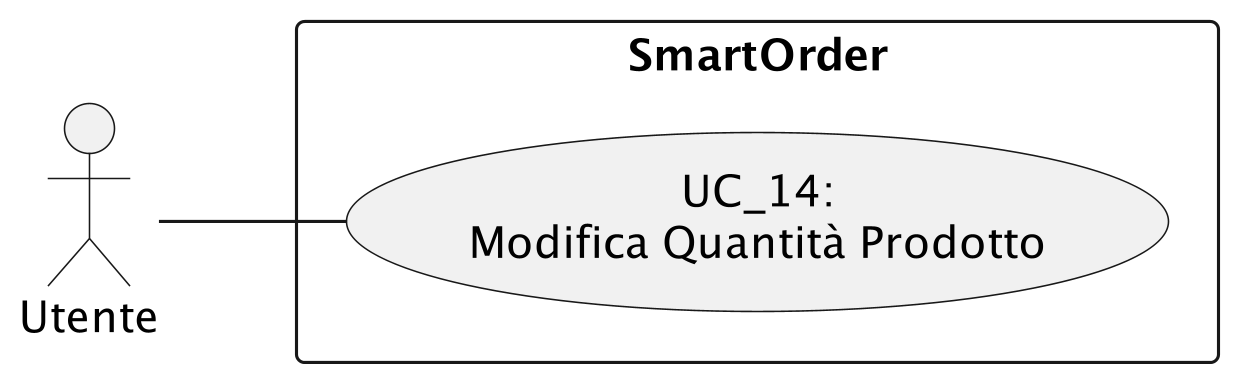
\includegraphics[width=0.6\textwidth]{uc-14.png}
    \caption{UC\_14: Modifica Quantità Prodotto in Carrello}
\end{figure}

\begin{itemize}
    \item \textbf{Attore Principale}: Utente
    \item \textbf{User Story}: Come Utente, voglio alterare il numero di articoli per rettificare i volumi in base alle mie nuove esigenze operative.
    \item \textbf{Scenario Principale}: 
    \begin{enumerate}
        \item L'Utente fornisce il nuovo dato utilizzando strumenti incrementali/decrementali o agendo per sovrascrittura testuale diretta.
        \item L'Utente agisce sull'elemento risolutivo delegato al salvataggio (es. icona di conferma).
    \end{enumerate}
    \item \textbf{Precondizioni}:
    \begin{itemize}
        \item Il blocco testuale risulta abilitato alla ricezione eventi (tramite \hyperref[uc_13.3]{UC\_13.3}).
    \end{itemize}
    \item \textbf{Postcondizioni}:
    \begin{itemize}
        \item La nuova istanza numerica viene consolidata nel database di sessione, sovrascrivendo l'originaria. L'interfaccia della riga viene ricongelata.
    \end{itemize}
    \item \textbf{Estensioni}:
    \begin{itemize}
        \item Fornitura dato anomalo $\rightarrow$ Il sistema invalida immissioni negative o alfabetico/simboliche attuando un respingimento e forzando la correzione numerica.
        \item Annullamento volontario $\rightarrow$ L'Utente innesca il comando di aborto (Undo). Il sistema esegue il rollback visivo dismettendo il dato pendente e ripristinando il numero ufficiale validato in precedenza.
    \end{itemize}
\end{itemize}

% -------------------------------------------------------------------

\subsection{UC\_15: Conferma Ordine (Trasmissione Esterna)}
\label{uc_15}

\begin{figure}[H]
    \centering 
    
\includegraphics[width=0.8\textwidth]{uc-15.png}
    \caption{UC\_15: Conferma Ordine}
\end{figure}

\begin{itemize}
    \item \textbf{Attore Principale}: Cliente
    \item \textbf{User Story}: Come Cliente, ritenendomi soddisfatto della lista creata, voglio richiedere la sottomissione formale della richiesta, affinché venga processata a livello commerciale e logistico dal fornitore.
    \item \textbf{Scenario Principale}: 
    \begin{enumerate}
        \item Il Cliente richiede formalmente la finalizzazione attivando il controllo primario di checkout.
        \item Il frontend confeziona il payload dell'ordine e lo invia al backend locale per un'analisi di validità.
        \item Trasmissione dati transazionali al Sistema ERP $\rightarrow$ Vedi \hyperref[uc_15.2]{UC\_15.2}
    \end{enumerate}
    \item \textbf{Precondizioni}:
    \begin{itemize}
        \item La lista articoli conta almeno una referenza valida a database.
        \item Non vi sono alterazioni o ticket di teleassistenza in stato pendente o sospeso per l'utenza corrente.
    \end{itemize}
    \item \textbf{Postcondizioni}:
    \begin{itemize}
        \item L'array di sessione del carrello viene destituito e i log semantici AI isolati per il tracciamento. Il Cliente viene instradato tramite routing automatico alla dashboard dello Storico Ordini (\hyperref[uc_16]{UC\_16}).
    \end{itemize}
    \item \textbf{Inclusioni}:
    \begin{itemize}
        \item \hyperref[uc_15.2]{UC\_15.2}
    \end{itemize}
    \item \textbf{Estensioni}:
    \begin{itemize}
        \item La validazione backend solleva eccezioni insormontabili $\rightarrow$ Vedi \hyperref[uc_15.1]{UC\_15.1}
    \end{itemize}
    \item \textbf{Trigger}: Intenzione conclamata del Cliente di passare all'acquisizione logistica.
\end{itemize}

\subsubsection{UC\_15.1: Blocco per violazione logica di business}
\label{uc_15.1}
\begin{itemize}
    \item \textbf{Attore Principale}: Cliente
    \item \textbf{Scenario Principale}: Il sistema backend incrocia i codici SKU del payload con le tabelle master ERP e riscontra un fallimento critico dovuto a incompatibilità assortimentale (es. prodotto escluso, oppure inventory in stato sospeso).
    \item \textbf{Postcondizioni}: Il processo di packaging e invio esterno decade. Il routing viene annullato e il Cliente viene mantenuto nell'area Carrello, dove le righe incriminate vengono marcate con un flag d'allarme affinché il Cliente provveda obbligatoriamente alla loro rimozione manuale.
\end{itemize}

\subsubsection{UC\_15.2: Invio al Sistema Esterno ERP}
\label{uc_15.2}
\begin{itemize}
    \item \textbf{Attori Principali}: Cliente, Sistema ERP (Attore Esterno)
    \item \textbf{Scenario Principale}:
    \begin{enumerate}
        \item Il backend della webapp compila l'intera architettura dati dell'ordine formattandola in un file strutturato.
        \item La piattaforma trasmette il file o lo deposita attivamente in un bucket/storage di interfaccia accessibile al dominio gestionale aziendale.
        \item Il Sistema ERP acquisisce i dati in ricezione passiva.
    \end{enumerate}
    \item \textbf{Postcondizioni}: I dati di carrello fuoriescono dal perimetro di competenza della webapp e acquisiscono rilevanza fiscale, contabile ed economica esclusivamente sotto l'egida infrastrutturale dell'ERP esterno (che ne elaborerà fatturazione e prezzi dedicati).
\end{itemize}

% ==========================================
% GRUPPO D: STORICO CLIENTE E ASSISTENZA
% ==========================================

\subsection{UC\_16: Visualizzazione Storico Ordini}
\label{uc_16}

\begin{figure}[H]
    \centering 
    
\includegraphics[width=0.8\textwidth]{uc-16.png}
    \caption{UC\_16: Visualizzazione Storico Ordini}
\end{figure}

\begin{itemize}
    \item \textbf{Attore Principale}: Cliente
    \item \textbf{User Story}: Come Cliente autenticato, voglio accedere a una lista cronologica di tutti gli ordini che ho effettuato in passato, affinché io possa consultare i miei volumi di acquisto e ritrovare specifiche transazioni.
    \item \textbf{Scenario Principale}: 
    \begin{enumerate}
        \item Il Cliente richiede l'accesso all'area dedicata allo storico tramite l'apposito comando di navigazione.
        \item Il sistema interroga il database locale e renderizza l'elenco degli ordini associati all'utenza, applicando un ordinamento cronologico discendente.
        \item Per ogni ordine esposto, il sistema genera una sintesi visiva comprendente:
        \begin{itemize}
            \item L'esposizione delle coordinate strutturali $\rightarrow$ Include: \hyperref[uc_00.3]{UC\_00.3}
            \item L'esposizione della sintesi quantitativa globale $\rightarrow$ Vedi \hyperref[uc_16.1]{UC\_16.1}
            \item L'esposizione di un'anteprima limitata degli articoli $\rightarrow$ Vedi \hyperref[uc_16.2]{UC\_16.2}
        \end{itemize}
    \end{enumerate}
    \item \textbf{Precondizioni}:
    \begin{itemize}
        \item Il sistema è online e l'Utente possiede una sessione attiva con privilegi di Cliente.
        \item Esiste almeno un record storico (anche vuoto) associato all'ID del Cliente nel database della piattaforma.
    \end{itemize}
    \item \textbf{Postcondizioni}:
    \begin{itemize}
        \item L'elenco viene mostrato a schermo. Se il Cliente proviene da una finalizzazione appena conclusa (tramite \hyperref[uc_15]{UC\_15}), il record in cima alla lista appare transitoriamente evidenziato per confermare il successo del checkout.
    \end{itemize}
    \item \textbf{Inclusioni}:
    \begin{itemize}
        \item \hyperref[uc_00.3]{UC\_00.3}, \hyperref[uc_16.1]{UC\_16.1}, \hyperref[uc_16.2]{UC\_16.2}
    \end{itemize}
    \item \textbf{Estensioni}:
    \begin{itemize}
        \item Il Cliente comanda lo scaricamento di un report tabellare $\rightarrow$ Vedi \hyperref[uc_16.3]{UC\_16.3}
    \end{itemize}
    \item \textbf{Trigger}: Navigazione volontaria del Cliente verso la rotta "Storico".
\end{itemize}

\subsubsection{UC\_16.1: Esposizione sintesi quantitativa (Totale Prodotti)}
\label{uc_16.1}
\begin{itemize}
    \item \textbf{Attore Principale}: Cliente
    \item \textbf{Scenario Principale}: A corredo delle coordinate temporali (\hyperref[uc_00.3]{UC\_00.3}), il sistema esegue un conteggio delle referenze uniche inserite in quell'ordine specifico e ne mostra il totale logico a video.
    \item \textbf{Postcondizioni}: L'informazione aggregata sui volumi della transazione è immediatamente leggibile senza necessità di espandere il dettaglio.
\end{itemize}

\subsubsection{UC\_16.2: Visualizzazione anteprima prodotti (Compatta)}
\label{uc_16.2}
\begin{itemize}
    \item \textbf{Attore Principale}: Cliente
    \item \textbf{Scenario Principale}: Il sistema estrae un sottoinsieme dei primi articoli associati all'ordine (es. le prime 3 referenze per mantenere compatto il layout). Per ciascuno di essi espone esclusivamente la denominazione commerciale in formato testuale e il numero di unità ordinate.
    \item \textbf{Postcondizioni}: Il Cliente ottiene un riscontro visivo rapido sul contenuto dell'ordine pregresso.
\end{itemize}

\subsubsection{UC\_16.3: Download storico ordini (Export CSV\textsubscript{\textsc{g}})}
\label{uc_16.3}
\begin{itemize}
    \item \textbf{Attore Principale}: Cliente
    \item \textbf{Nota Requisito}: Questa funzionalità è classificata come requisito desiderabile.
    \item \textbf{Scenario Principale}: Il Cliente attiva il comando di esportazione dati presente nella dashboard dello storico. Il sistema compila l'elenco in un formato strutturato e ne avvia il download.
    \item \textbf{Postcondizioni}: Un file \textit{.csv} contenente i metadati estratti viene generato e salvato nel file system locale del dispositivo del Cliente.
\end{itemize}

% -------------------------------------------------------------------

\subsection{UC\_17: Ispezione Dettaglio Ordine (Lato Cliente)}
\label{uc_17}

\begin{figure}[H]
    \centering 
    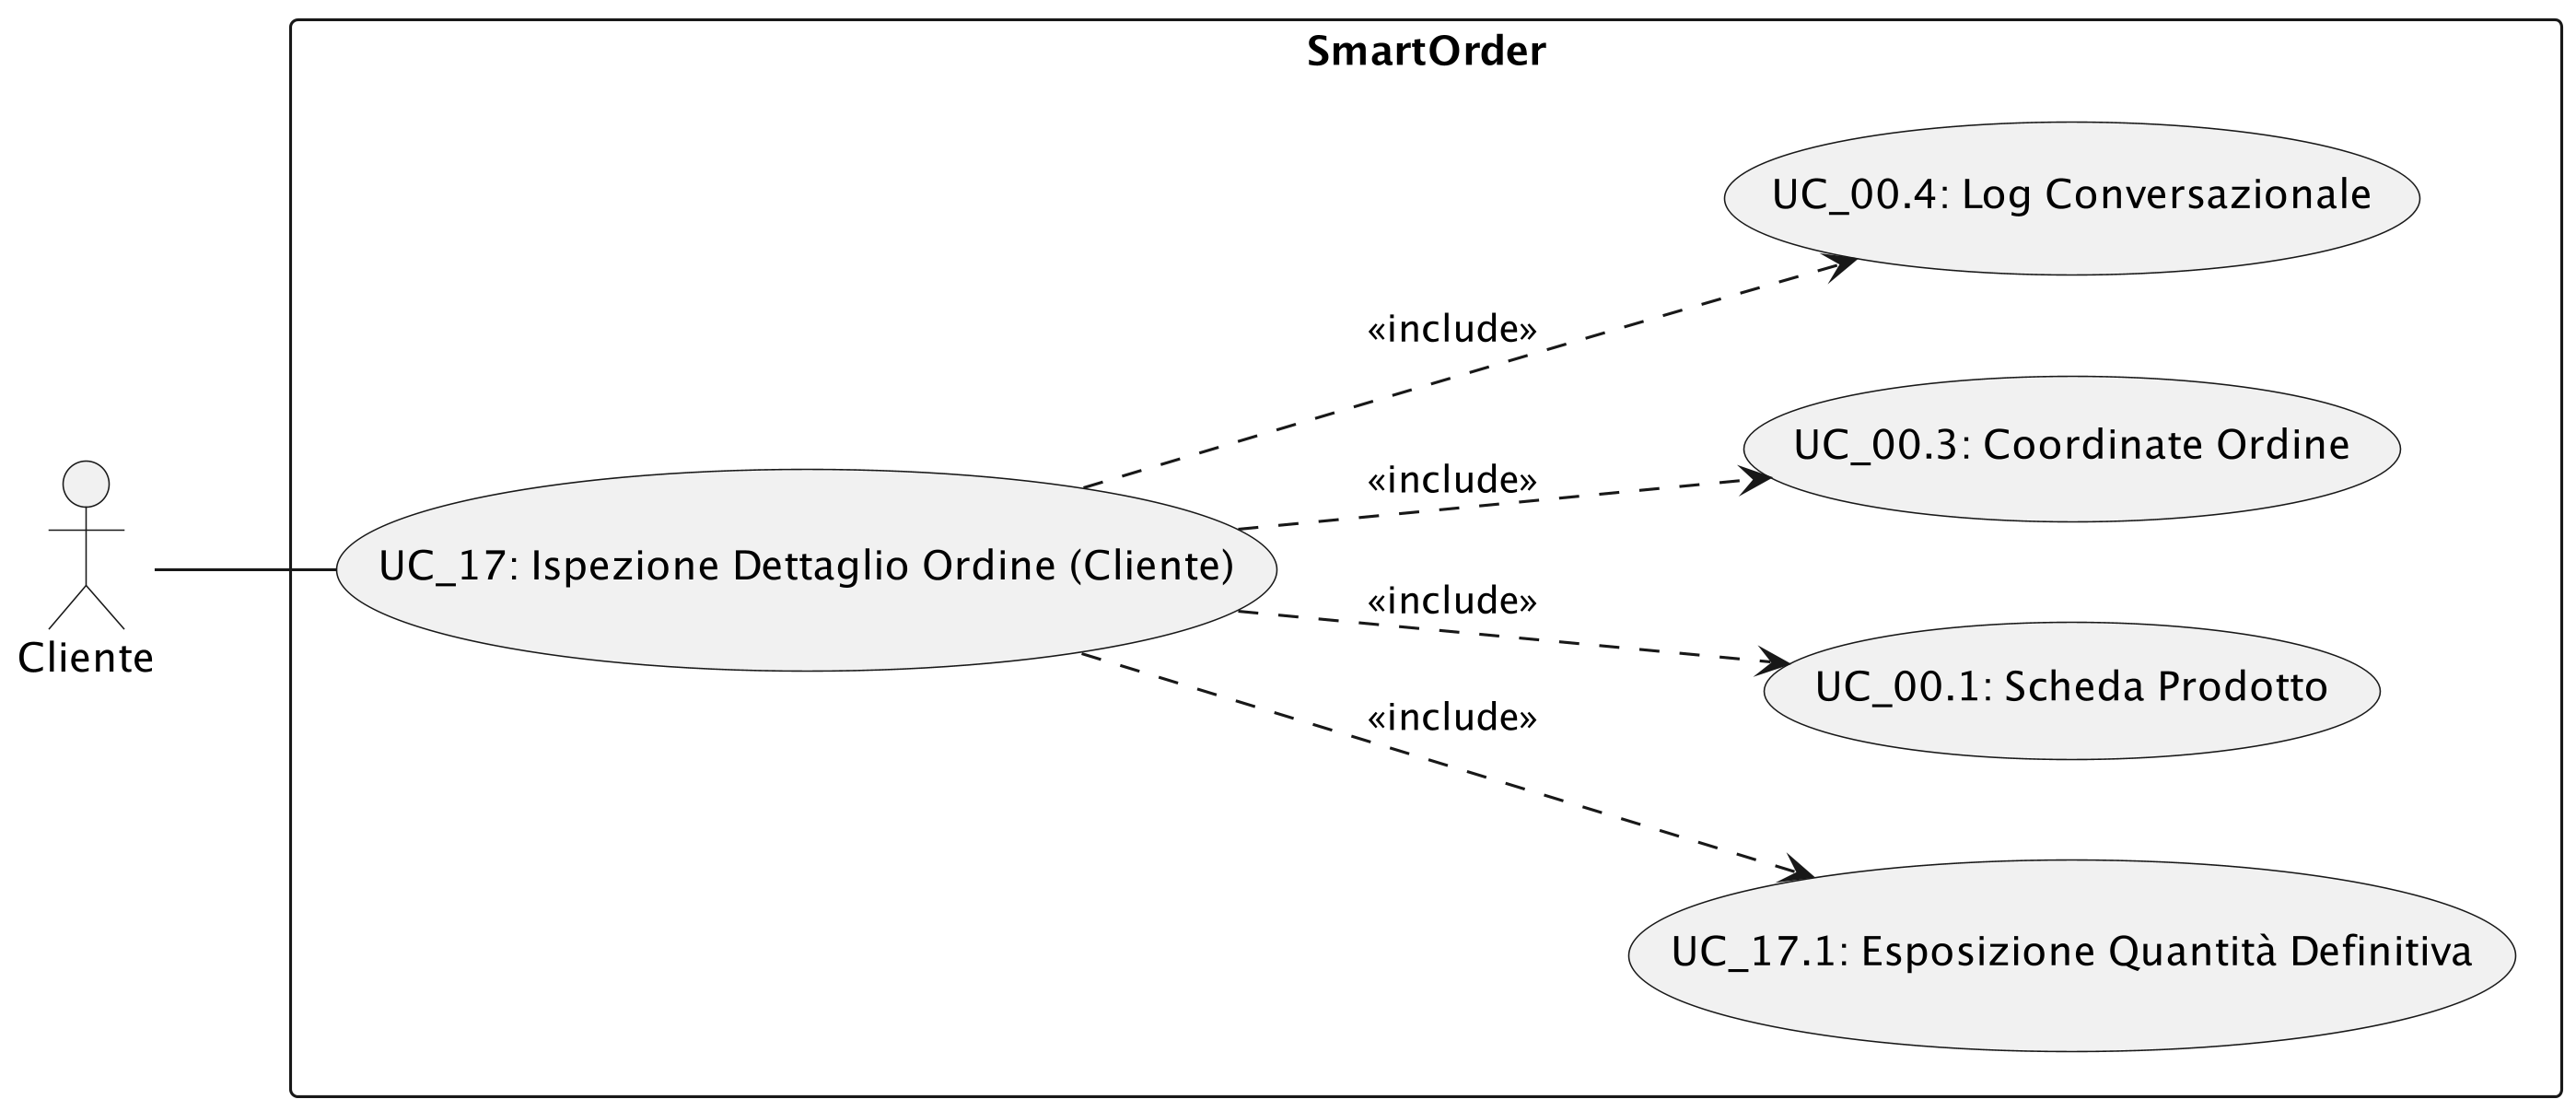
\includegraphics[width=0.8\textwidth]{uc-17.png}
    \caption{UC\_17: Visualizzazione Dettaglio Ordine}
\end{figure}

\begin{itemize}
    \item \textbf{Attore Principale}: Cliente
    \item \textbf{User Story}: Come Cliente, selezionando un ordine pregresso, voglio accedere a una vista approfondita che mi mostri l'elenco completo dei prodotti acquistati e la cronologia della conversazione che ha generato quel carrello.
    \item \textbf{Scenario Principale}: 
    \begin{enumerate}
        \item Il Cliente attiva il comando di espansione su uno specifico blocco riepilogativo dello Storico (\hyperref[uc_16]{UC\_16}).
        \item Il sistema istanzia la vista di dettaglio dedicata alla transazione.
        \item Il sistema espone le coordinate cardinali per inquadrare il documento $\rightarrow$ Include: \hyperref[uc_00.3]{UC\_00.3}
        \item Il sistema inietta il log storico della conversazione $\rightarrow$ Include: \hyperref[uc_00.4]{UC\_00.4}
        \item Per ogni articolo consolidato in quel checkout, il sistema ne espone la scheda anagrafica $\rightarrow$ Include: \hyperref[uc_00.1]{UC\_00.1}
        \item Per ogni articolo, viene affiancata la quantità storicizzata $\rightarrow$ Vedi \hyperref[uc_17.1]{UC\_17.1}
    \end{enumerate}
    \item \textbf{Precondizioni}:
    \begin{itemize}
        \item Il Cliente naviga nello Storico e attiva un record logicamente valido e associato al suo identificativo.
    \end{itemize}
    \item \textbf{Postcondizioni}:
    \begin{itemize}
        \item L'intero perimetro informativo dell'ordine (prodotti e chat) viene esposto in modalità di sola lettura (Read-Only). Nessuna operazione di modifica commerciale è ammessa, in quanto i dati risiedono già sotto l'autorità dell'ERP esterno.
    \end{itemize}
    \item \textbf{Inclusioni}:
    \begin{itemize}
        \item \hyperref[uc_00.1]{UC\_00.1}, \hyperref[uc_00.3]{UC\_00.3}, \hyperref[uc_00.4]{UC\_00.4}, \hyperref[uc_17.1]{UC\_17.1}
    \end{itemize}
    \item \textbf{Trigger}: Interazione fisica sul record di un ordine in elenco.
\end{itemize}

\subsubsection{UC\_17.1: Esposizione Quantità Definitiva}
\label{uc_17.1}
\begin{itemize}
    \item \textbf{Attore Principale}: Cliente
    \item \textbf{Scenario Principale}: A integrazione dei metadati logistici forniti da \hyperref[uc_00.1]{UC\_00.1}, il sistema espone il numero esatto di unità inviate al gestionale per quello specifico prodotto al momento del checkout.
    \item \textbf{Postcondizioni}: Il valore numerico viene renderizzato in formato testo, privo di qualsiasi controllo di iterazione incrementale o decrementale (impossibilità di alterazione).
\end{itemize}

% -------------------------------------------------------------------

\subsection{UC\_18: Gestione Assistenza Ticket (Lato Cliente)}
\label{uc_18}
 
\begin{figure}[H]
    \centering 
    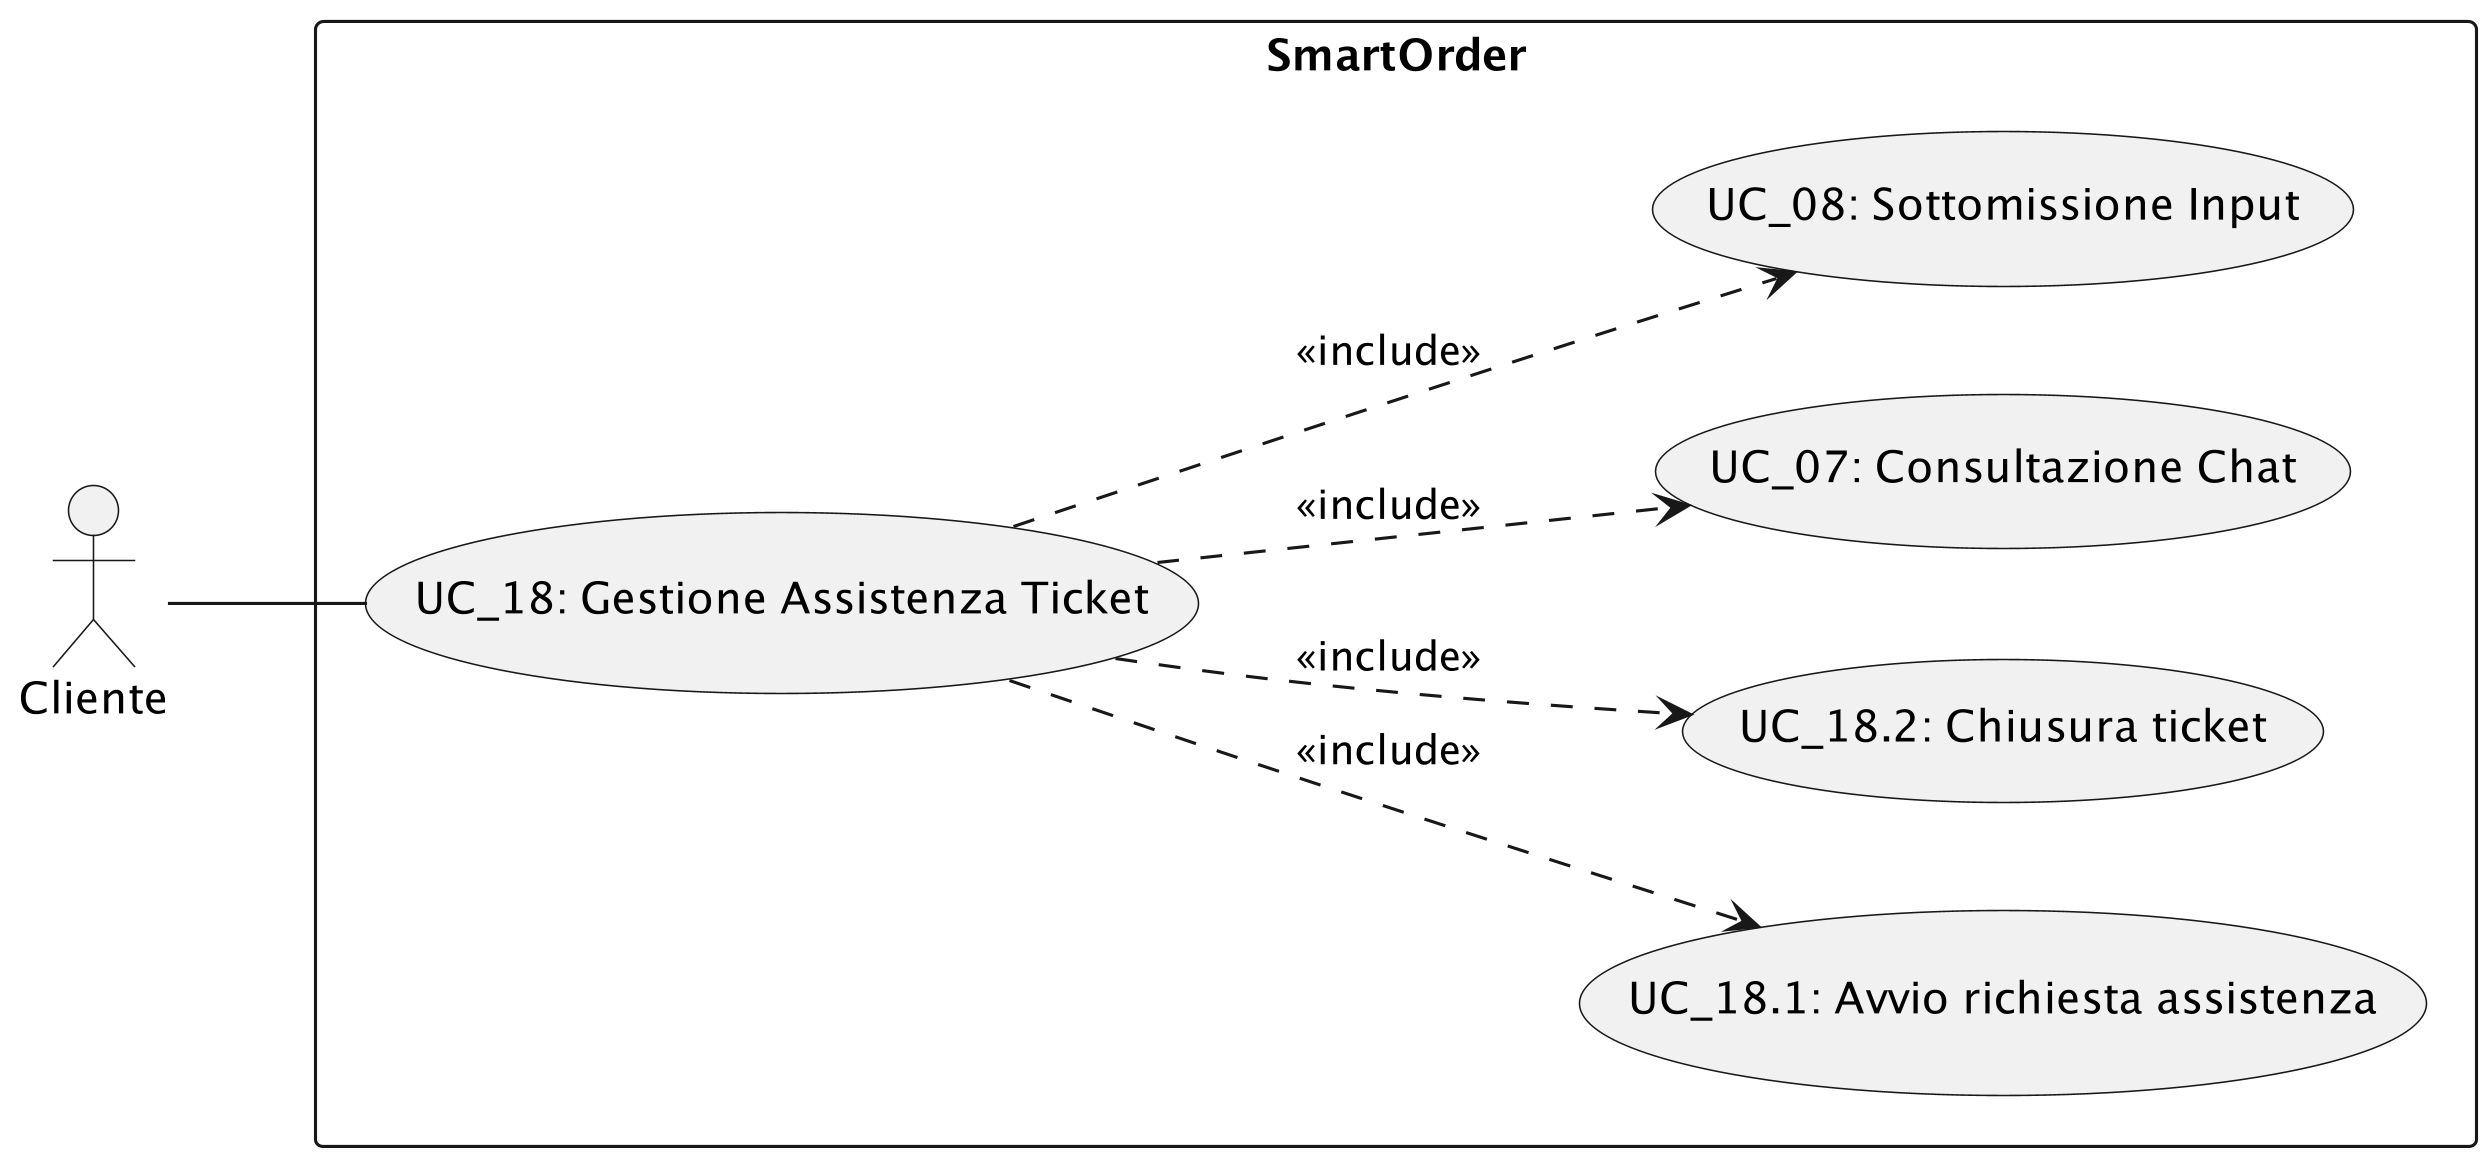
\includegraphics[width=1\textwidth]{uc-18.png}
    \caption{UC\_18: Assistenza Lato Cliente}
\end{figure}

\begin{itemize}
    \item \textbf{Attore Principale}: Cliente
    \item \textbf{User Story}: Come Cliente, se mi trovo bloccato a causa di incomprensioni dell'AI, voglio poter innescare un processo di escalation\textsubscript{\textsc{g}} per richiedere l'intervento di un operatore umano che subentri nel controllo del mio carrello.
    \item \textbf{Scenario Principale}: 
    \begin{enumerate}
        \item Avvio richiesta formale di assistenza (Escalation) $\rightarrow$ Vedi \hyperref[uc_18.1]{UC\_18.1}
        \item Il Cliente sfrutta l'interfaccia standard per l'interazione bidirezionale con l'Operatore subentrato $\rightarrow$ Include: \hyperref[uc_07]{UC\_07}, \hyperref[uc_08]{UC\_08}
        \item Conclusione del supporto e chiusura $\rightarrow$ Vedi \hyperref[uc_18.2]{UC\_18.2}
    \end{enumerate}
    \item \textbf{Precondizioni}:
    \begin{itemize}
        \item Il Cliente si trova nell'interfaccia di composizione attiva dell'ordine.
        \item Non ci sono altri ticket di assistenza attualmente pendenti per la medesima sessione logica.
    \end{itemize}
    \item \textbf{Postcondizioni}:
    \begin{itemize}
        \item La gestione semantica autonoma dell'LLM viene temporaneamente sospesa. L'Operatore remoto riceve un token di Lock che gli conferisce privilegi di manipolazione asincrona sul carrello in esame.
    \end{itemize}
    \item \textbf{Inclusioni}:
    \begin{itemize}
        \item \hyperref[uc_07]{UC\_07}, \hyperref[uc_08]{UC\_08}, \hyperref[uc_18.1]{UC\_18.1}, \hyperref[uc_18.2]{UC\_18.2}
    \end{itemize}
\end{itemize}

\subsubsection{UC\_18.1: Avvio richiesta assistenza (Escalation)}
\label{uc_18.1}
\begin{itemize}
    \item \textbf{Attore Principale}: Cliente
    \item \textbf{Scenario Principale}:
    \begin{enumerate}
        \item Il Cliente innesca il comando logico di richiesta assistenza.
        \item Il sistema inserisce la richiesta (sotto forma di Ticket) nella coda d'attesa del backoffice Operatori.
    \end{enumerate}
    \item \textbf{Precondizioni}: L'Intelligenza Artificiale ha concluso l'elaborazione dell'ultimo pacchetto testuale (se presente).
    \item \textbf{Postcondizioni}: L'interfaccia aggiorna la toolbar dei comandi (commutando l'azione principale in "Chiudi ticket" e disabilitando il "Reset Sessione"). Il sistema inietta nel flusso un messaggio standard di cortesia comunicando la messa in attesa.
    \item \textbf{Trigger}: Attivazione intenzionale del comando di richiesta aiuto.
\end{itemize}

\subsubsection{UC\_18.2: Chiusura ticket (Lato Cliente)}
\label{uc_18.2}
\begin{itemize}
    \item \textbf{Attore Principale}: Cliente
    \item \textbf{Scenario Principale}:
    \begin{enumerate}
        \item Il Cliente attiva il comando di chiusura del ticket, ritenendo risolta l'anomalia o non necessitando più di supporto.
        \item Il sistema destituisce il supporto condiviso, forza il rilascio del Lock operatore e chiude la sessione dedicata nel backoffice.
    \end{enumerate}
    \item \textbf{Precondizioni}: Il ticket si trova formalmente in stato "Aperto" o "In lavorazione".
    \item \textbf{Postcondizioni}: I controlli dell'interfaccia tornano allo stato predefinito. Il controllo degli input conversazionali viene riconsegnato in toto al dominio dell'Intelligenza Artificiale e un log di sistema certifica in chat l'avvenuta dismissione dell'intervento umano.
    \item \textbf{Trigger}: Attivazione del comando di dismissione assistenza.
\end{itemize}

% ==========================================
% GRUPPO E: NAVIGAZIONE E FILTRI (OPERATORE)
% ==========================================

\subsection{UC\_19: Navigazione Viste Operative}
\label{uc_19}

\begin{figure}[H]
    \centering 
    
\includegraphics[width=0.8\textwidth]{uc-19.png}
    \caption{UC\_19: Navigazione Viste Operative}
\end{figure}

\begin{itemize}
    \item \textbf{Attore Principale}: Operatore
    \item \textbf{User Story}: Come Operatore autenticato, voglio poter navigare tra le diverse sezioni principali del backoffice tramite comandi rapidi di selezione posti nella sidebar.
    \item \textbf{Scenario Principale}: 
    \begin{enumerate}
        \item L'Operatore sceglie di navigare verso la dashboard "Ticket aperti" $\rightarrow$ Vedi \hyperref[uc_19.1]{UC\_19.1}
        \item L'Operatore sceglie di navigare verso lo storico "Ordini" $\rightarrow$ Vedi \hyperref[uc_19.2]{UC\_19.2}
        \item L'Operatore sceglie di navigare verso il modulo "Ottimizzazione AI" $\rightarrow$ Vedi \hyperref[uc_19.3]{UC\_19.3}
    \end{enumerate}
    \item \textbf{Precondizioni}:
    \begin{itemize}
        \item L'Utente è autenticato a sistema con i privilegi di accesso del ruolo "Operatore".
        \item L'interfaccia globale (layout principale) è caricata e i controlli di navigazione (routing) sono abilitati.
    \end{itemize}
    \item \textbf{Postcondizioni}:
    \begin{itemize}
        \item Il sistema destituisce dal DOM\textsubscript{\textsc{g}} (Document Object Model) i componenti della vista corrente e istanzia gli elementi, i filtri e le tabelle associati alla nuova vista richiesta.
    \end{itemize}
    \item \textbf{Specializzazioni}:
    \begin{itemize}
        \item \hyperref[uc_19.1]{UC\_19.1}, \hyperref[uc_19.2]{UC\_19.2}, \hyperref[uc_19.3]{UC\_19.3}
    \end{itemize}
    \item \textbf{Trigger}: L'Operatore interagisce attivamente con un comando di routing per transitare verso un differente dominio logico del backoffice.
\end{itemize}

\subsubsection{UC\_19.1: Navigazione a "Ticket aperti"}
\label{uc_19.1}
\begin{itemize}
    \item \textbf{Attore Principale}: Operatore
    \item \textbf{Scenario Principale}: L'Operatore attiva il comando di routing relativo alla coda di assistenza tecnica.
    \item \textbf{Precondizioni}: L'Operatore non si trova già all'interno di questa specifica vista.
    \item \textbf{Postcondizioni}: Il sistema evidenzia la selezione corrente sul menu e innesca il caricamento della tabella delle richieste pendenti (\hyperref[uc_23]{UC\_23}).
\end{itemize}

\subsubsection{UC\_19.2: Navigazione a "Ordini"}
\label{uc_19.2}
\begin{itemize}
    \item \textbf{Attore Principale}: Operatore
    \item \textbf{Scenario Principale}: L'Operatore attiva il comando di routing relativo alla dashboard transazionale.
    \item \textbf{Precondizioni}: L'Operatore non si trova già all'interno di questa specifica vista.
    \item \textbf{Postcondizioni}: Il sistema evidenzia la selezione sul menu e innesca il caricamento della tabella dello Storico Ordini globale (\hyperref[uc_25]{UC\_25}).
\end{itemize}

\subsubsection{UC\_19.3: Navigazione a "Ottimizzazione AI"}
\label{uc_19.3}
\begin{itemize}
    \item \textbf{Attore Principale}: Operatore
    \item \textbf{Scenario Principale}: L'Operatore attiva il comando di routing relativo al modulo Human-in-the-Loop per l'addestramento.
    \item \textbf{Precondizioni}: L'Operatore non si trova già all'interno di questa specifica vista.
    \item \textbf{Postcondizioni}: Il sistema evidenzia la selezione sul menu e innesca il caricamento della tabella di telemetria semantica (\hyperref[uc_27]{UC\_27}).
\end{itemize}

% -------------------------------------------------------------------
\subsection*{Filtri tabellari (UC\_20, UC\_21, UC\_22, UC\_28)}

\begin{figure}[H] 
    \centering 
    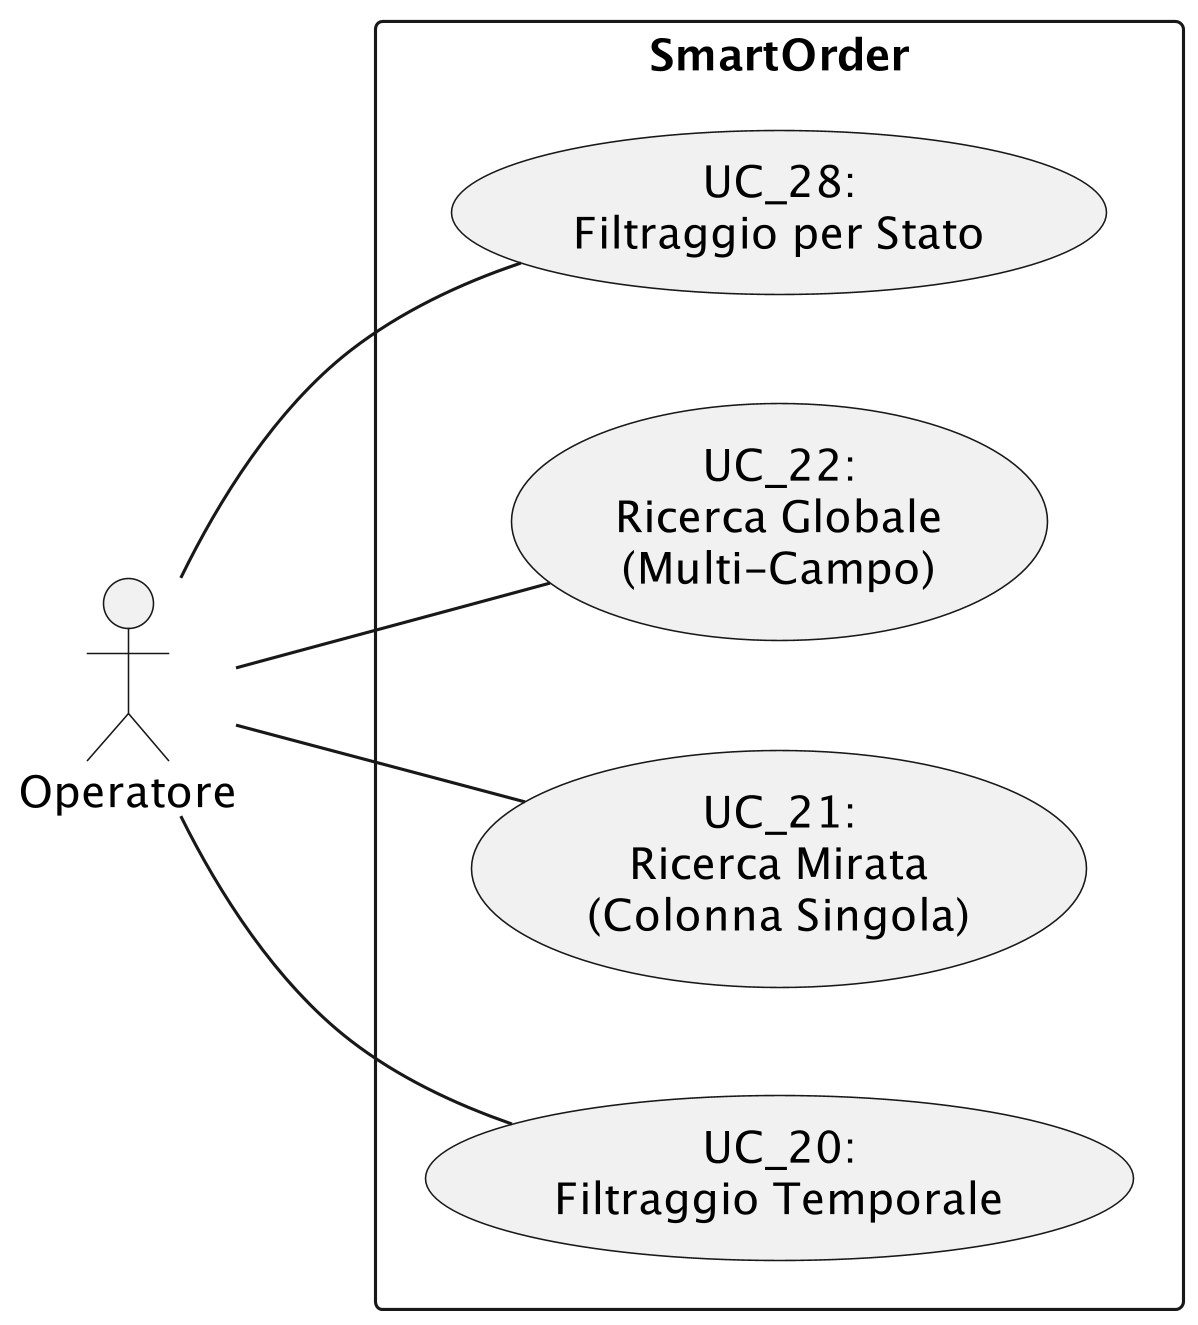
\includegraphics[width=0.6\textwidth]{uc-20.png}
    \caption{UC\_20: Filtraggio Temporale dei Record}
\end{figure}


\subsection{UC\_20: Filtraggio Temporale dei Record}
\label{uc_20}

\begin{itemize}
    \item \textbf{Attore Principale}: Operatore
    \item \textbf{User Story}: Come Operatore, voglio poter isolare i record esposti in base a un periodo di tempo specifico, affinché io possa focalizzare l'analisi visiva su un dominio cronologico strettamente delimitato.
    \item \textbf{Scenario Principale}: 
    \begin{enumerate}
        \item L'Operatore impone un vincolo temporale (es. data di inizio e/o data di fine) avvalendosi dell'apposito controllo logico di filtraggio.
        \item Il sistema cattura il parametro, avvia l'interrogazione sul set di dati e destituisce dalla visualizzazione tutti i record non compresi nell'intervallo indicato.
    \end{enumerate}
    \item \textbf{Precondizioni}:
    \begin{itemize}
        \item La vista tabellare corrente (\hyperref[uc_23]{UC\_23}, \hyperref[uc_25]{UC\_25} o \hyperref[uc_27]{UC\_27}) prevede l'accesso ai moduli di filtro su campi Data/Timestamp ed è regolarmente istanziata.
    \end{itemize}
    \item \textbf{Postcondizioni}:
    \begin{itemize}
        \item L'interfaccia si aggiorna in tempo reale omettendone i risultati estranei e mostrando esclusivamente le occorrenze pertinenti al parametro cronologico applicato.
    \end{itemize}
    \item \textbf{Trigger}: Necessità dell'Operatore di sfoltire i dati visibili isolando una precisa finestra di tempo.
\end{itemize}

% -------------------------------------------------------------------

\subsection{UC\_21: Ricerca Mirata a Colonna Singola}
\label{uc_21}

\begin{itemize}
    \item \textbf{Attore Principale}: Operatore
    \item \textbf{User Story}: Come Operatore, voglio poter cercare un record definendo con precisione l'unica colonna della tabella in cui il sistema deve eseguire l'ispezione testuale.
    \item \textbf{Scenario Principale}: 
    \begin{enumerate}
        \item L'Operatore seleziona l'attributo logico bersaglio (es. ID Ordine, Cliente) imponendo il vincolo tramite l'apposito selettore.
        \item L'Operatore immette la sequenza testuale di ricerca all'interno dell'input associato.
        \item Il sistema intercetta la stringa ed estrae istantaneamente i soli record la cui colonna corrispondente contenga un \textit{match} semantico valido.
    \end{enumerate}
    \item \textbf{Precondizioni}:
    \begin{itemize}
        \item La vista tabellare corrente (\hyperref[uc_23]{UC\_23} o \hyperref[uc_25]{UC\_25}) supporta l'esposizione di filtri vincolati ai singoli campi.
    \end{itemize}
    \item \textbf{Postcondizioni}:
    \begin{itemize}
        \item La tabella dati si restringe mostrando esclusivamente le occorrenze pertinenti. La cancellazione totale dell'input testuale da parte dell'Operatore annulla l'operazione di sfoltimento, ripristinando il set completo.
    \end{itemize}
    \item \textbf{Trigger}: Immissione fisica di dati all'interno del modulo di ricerca mirata.
\end{itemize}

% -------------------------------------------------------------------

\subsection{UC\_22: Esecuzione Ricerca Globale Multi-Campo}
\label{uc_22}

\begin{itemize}
    \item \textbf{Attore Principale}: Operatore
    \item \textbf{User Story}: Come Operatore, voglio usufruire di una ricerca unificata che individui le mie occorrenze in modo distribuito, sondando in parallelo qualsiasi colonna testuale disponibile.
    \item \textbf{Scenario Principale}: 
    \begin{enumerate}
        \item L'Operatore compila il controllo testuale globale innescando il matching asincrono, senza imporre alcuna preselezione di colonna.
        \item L'algoritmo esegue una scansione parallela su tutti gli attributi testuali del recordset (logica \textit{OR}).
        \item Il sistema aggiorna dinamicamente la visualizzazione dei risultati a schermo.
    \end{enumerate}
    \item \textbf{Precondizioni}:
    \begin{itemize}
        \item La vista tabellare della telemetria AI (\hyperref[uc_27]{UC\_27}) è attiva, popolata e supporta l'esplorazione full-text asincrona.
    \end{itemize}
    \item \textbf{Postcondizioni}:
    \begin{itemize}
        \item La tabella dati si restringe mostrando le occorrenze secondo la massima tolleranza trasversale.
    \end{itemize}
    \item \textbf{Trigger}: Immissione di testo nel modulo di ricerca globale.
\end{itemize}

%-------------------------------------------

\subsection{UC\_28: Filtraggio Segnalazioni per Stato di Validazione}
\label{uc_28}

\begin{itemize}
    \item \textbf{Attore Principale}: Operatore
    \item \textbf{User Story}: Come Operatore, voglio poter isolare la visualizzazione dei log di telemetria AI in funzione del loro stadio di elaborazione (es. "Da gestire", "Accettate"), affinché io possa focalizzare l'analisi esclusivamente sui task pertinenti.
    \item \textbf{Scenario Principale}: 
    \begin{enumerate}
        \item L'Operatore esplora le opzioni di restrizione logica interagendo con il componente dedicato.
        \item L'Operatore impone l'ambito logico desiderato (es. "Da gestire") tramite il controllo a scelta.
        \item Il sistema avvia l'interrogazione interna e destituisce istantaneamente dalla visualizzazione tutti i record disallineati alla richiesta.
    \end{enumerate}
    \item \textbf{Precondizioni}:
    \begin{itemize}
        \item La dashboard "Ottimizzazione AI" (\hyperref[uc_27]{UC\_27}) è attiva e il sistema espone il modulo di filtro in cima alla tabella.
    \end{itemize}
    \item \textbf{Postcondizioni}:
    \begin{itemize}
        \item La tabella dati si restringe mostrando esclusivamente le occorrenze che soddisfano il parametro di stato selezionato. I record aventi attributo logico differente (es. "Rifiutato") restano nascosti e non recuperabili da interfaccia standard.
    \end{itemize}
    \item \textbf{Trigger}: Necessità dell'Operatore di sfoltire l'elenco dei log escludendo i record già processati o non rilevanti al momento.
\end{itemize}

% ==========================================
% GRUPPO F: GESTIONE TICKET APERTI (OPERATORE)
% ==========================================

\subsection{UC\_23: Visualizzazione Tabella "Ticket Aperti"}
\label{uc_23}

\begin{figure}[H]
    \centering 
    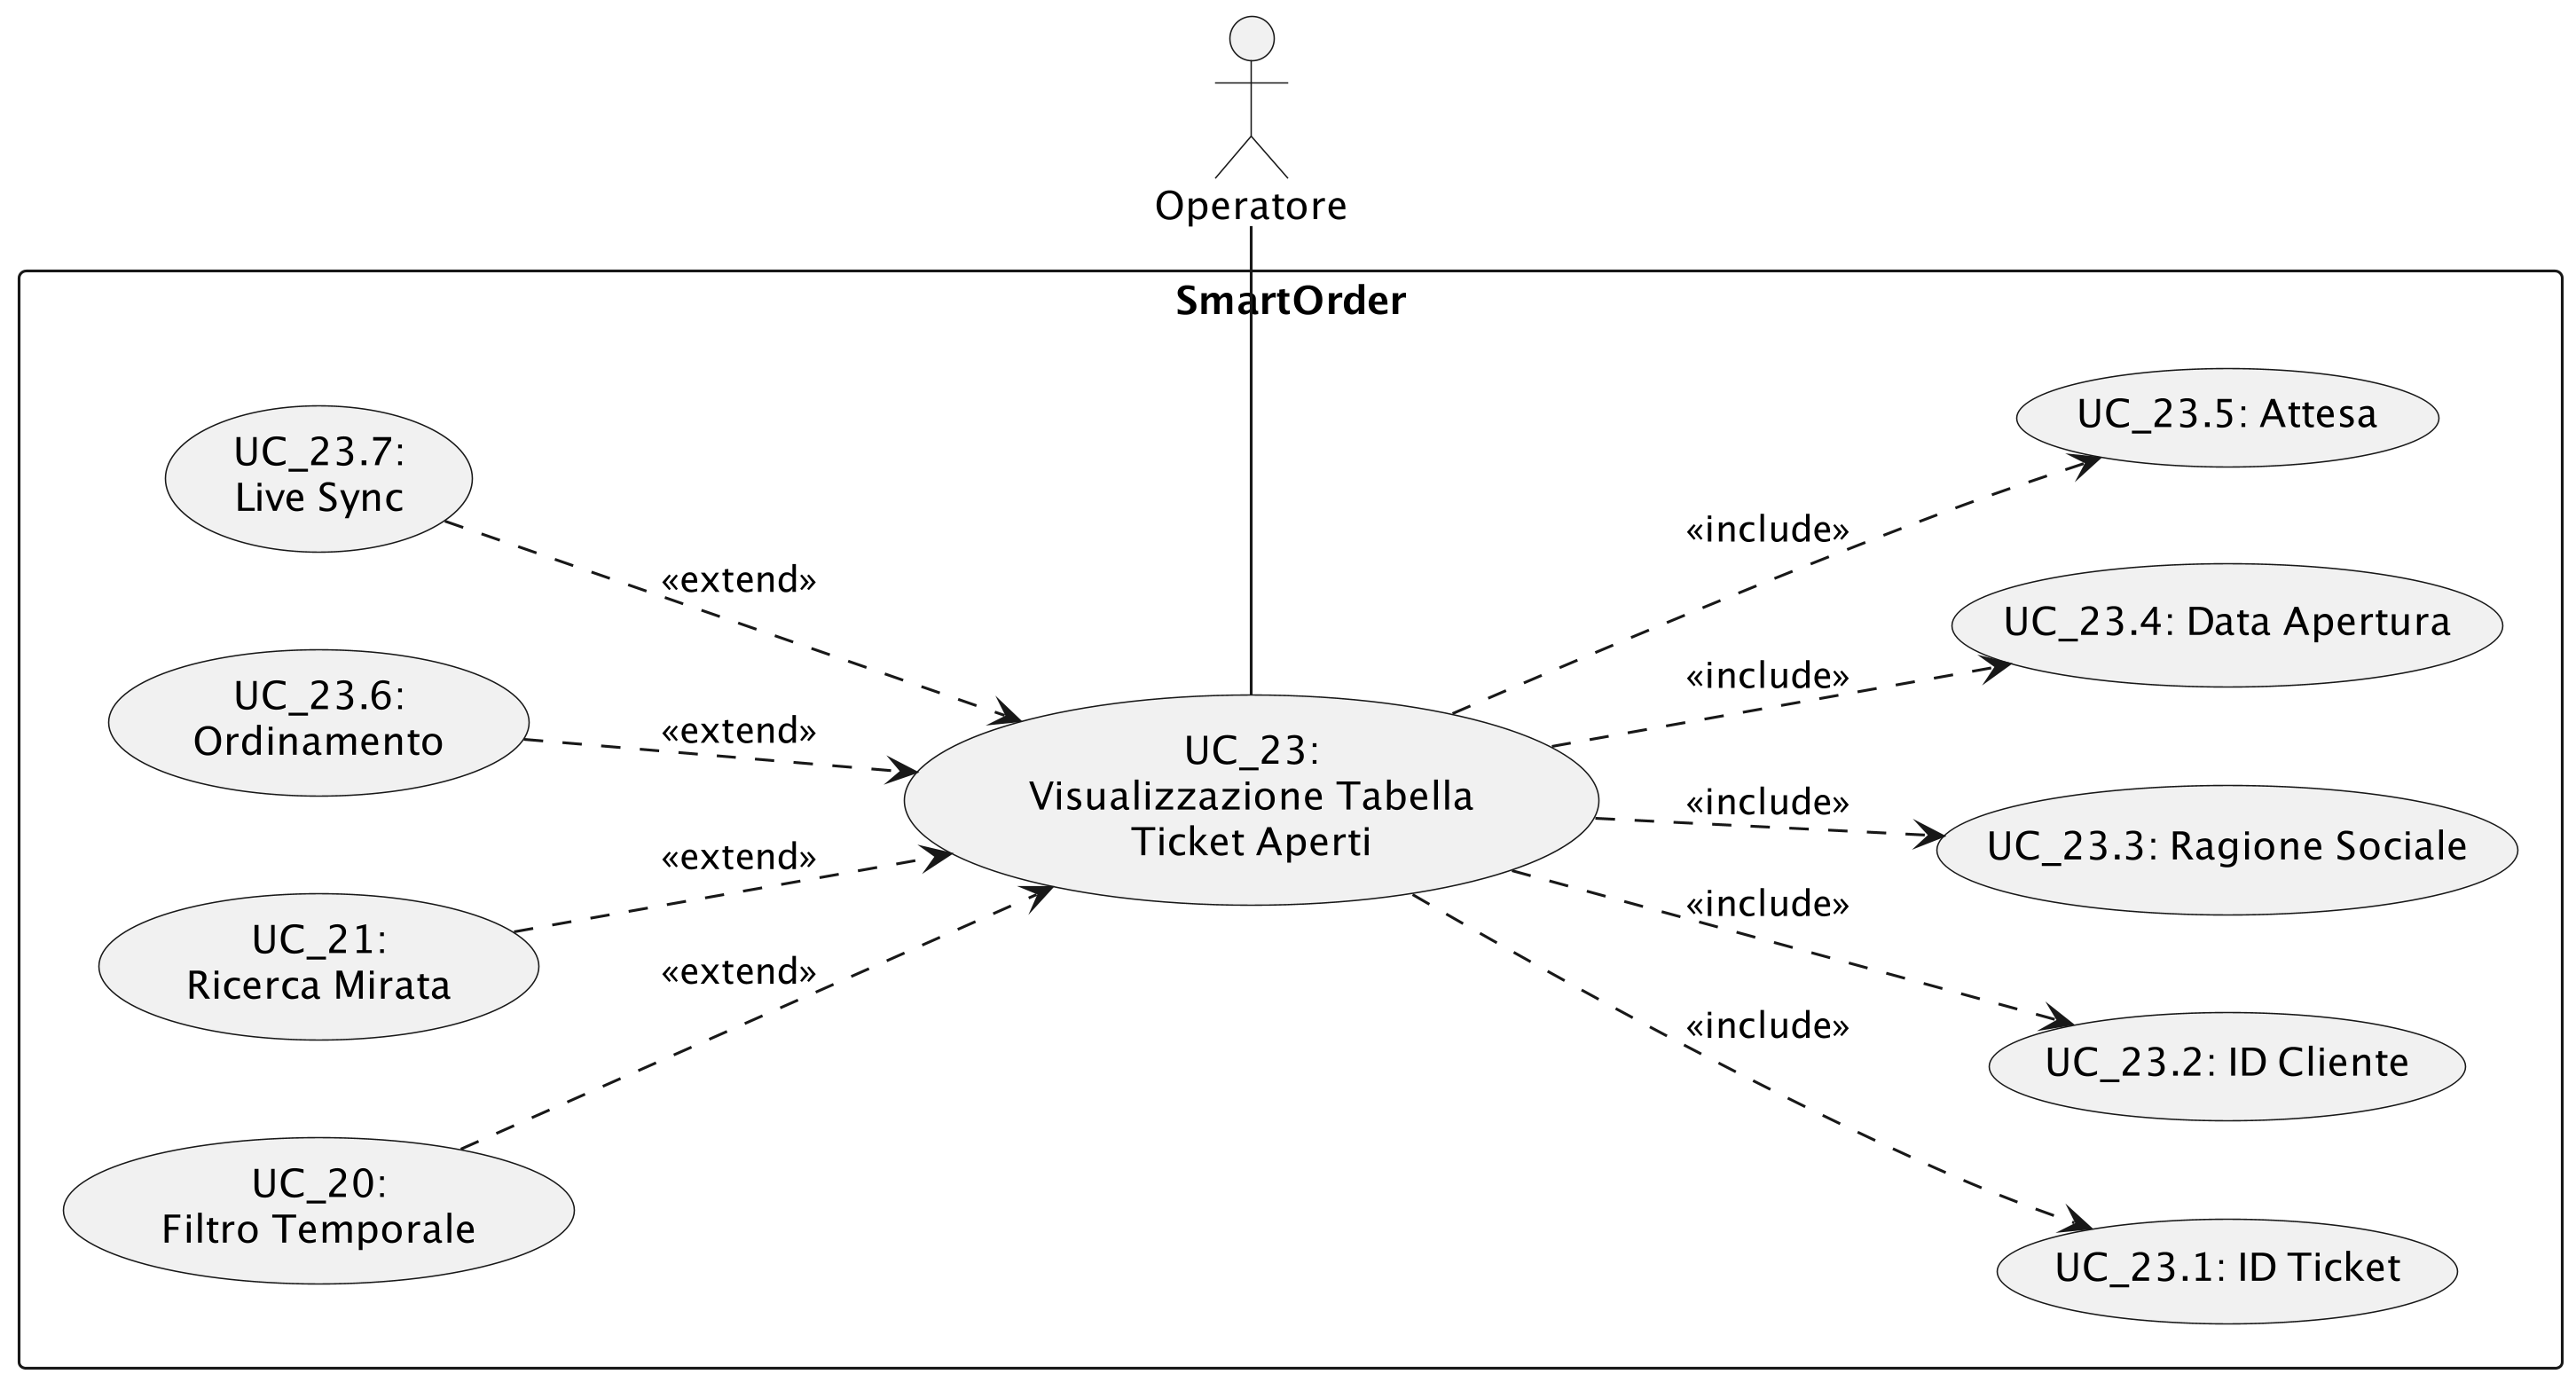
\includegraphics[width=0.8\textwidth]{uc-23.png}
    \caption{UC\_23: Visualizzazione Tabella "Ticket Aperti"}
\end{figure}

\begin{itemize}
    \item \textbf{Attore Principale}: Operatore
    \item \textbf{User Story}: Come Operatore, voglio visualizzare una tabella riepilogativa con tutte le richieste di assistenza ai carrelli attualmente in sospeso, affinché io possa valutarne le priorità d'intervento.
    \item \textbf{Scenario Principale}: 
    \begin{enumerate}
        \item Il sistema interroga il database locale e popola l'elenco delle richieste di escalation (Ticket) pendenti.
        \item Il sistema applica un ordinamento logico predefinito (discendente basato sul tempo di attesa), evidenziando il criterio attivo tramite apposito indicatore grafico nell'intestazione.
        \item Per ciascun record, esposizione ID Ticket $\rightarrow$ Vedi \hyperref[uc_23.1]{UC\_23.1}
        \item Per ciascun record, esposizione ID Cliente $\rightarrow$ Vedi \hyperref[uc_23.2]{UC\_23.2}
        \item Per ciascun record, esposizione Ragione Sociale $\rightarrow$ Vedi \hyperref[uc_23.3]{UC\_23.3}
        \item Per ciascun record, esposizione Data Apertura Ticket $\rightarrow$ Vedi \hyperref[uc_23.4]{UC\_23.4}
        \item Per ciascun record, esposizione Attesa differenziale $\rightarrow$ Vedi \hyperref[uc_23.5]{UC\_23.5}
    \end{enumerate}
    \item \textbf{Precondizioni}:
    \begin{itemize}
        \item L'Operatore ha validamente navigato verso la vista di competenza (tramite \hyperref[uc_19.1]{UC\_19.1}).
    \end{itemize}
    \item \textbf{Postcondizioni}:
    \begin{itemize}
        \item L'interfaccia presenta in modo reattivo l'elenco dei task, permettendo all'Operatore di far uso dei controlli di ricerca/filtro o di selezionare una riga per innescare l'ispezione (\hyperref[uc_24]{UC\_24}).
    \end{itemize}
    \item \textbf{Inclusioni}:
    \begin{itemize}
        \item \hyperref[uc_23.1]{UC\_23.1}, \hyperref[uc_23.2]{UC\_23.2}, \hyperref[uc_23.3]{UC\_23.3}, \hyperref[uc_23.4]{UC\_23.4}, \hyperref[uc_23.5]{UC\_23.5}
    \end{itemize}
    \item \textbf{Estensioni}:
    \begin{itemize}
        \item Inversione dinamica dell'ordinamento $\rightarrow$ Vedi \hyperref[uc_23.6]{UC\_23.6}
        \item Ricezione aggiornamento asincrono (Live Sync\textsubscript{\textsc{g}}) $\rightarrow$ Vedi \hyperref[uc_23.7]{UC\_23.7}
        \item Filtraggio Temporale dei Record $\rightarrow$ Extend: \hyperref[uc_20]{UC\_20}
        \item Ricerca Mirata a Colonna Singola $\rightarrow$ Extend: \hyperref[uc_21]{UC\_21}
    \end{itemize}
\end{itemize}

\subsubsection{UC\_23.1: Visualizzazione ID Ticket}
\label{uc_23.1}
\begin{itemize}
    \item \textbf{Attore Principale}: Operatore
    \item \textbf{Scenario Principale}: Il sistema preleva ed espone nella colonna preposta il codice alfanumerico univoco di sistema associato alla specifica richiesta di supporto.
\end{itemize}

\subsubsection{UC\_23.2: Visualizzazione ID Cliente}
\label{uc_23.2}
\begin{itemize}
    \item \textbf{Attore Principale}: Operatore
    \item \textbf{Scenario Principale}: Il sistema espone il codice anagrafico gestionale afferente al Cliente che ha innescato l'escalation.
\end{itemize}

\subsubsection{UC\_23.3: Visualizzazione Ragione Sociale}
\label{uc_23.3}
\begin{itemize}
    \item \textbf{Attore Principale}: Operatore
    \item \textbf{Scenario Principale}: Il sistema risolve la chiave esterna e preleva dalla tabella anagrafica locale la denominazione estesa dell'azienda, rendendola visibile in tabella.
\end{itemize}

\subsubsection{UC\_23.4: Visualizzazione Data Apertura Ticket}
\label{uc_23.4}
\begin{itemize}
    \item \textbf{Attore Principale}: Operatore
    \item \textbf{Scenario Principale}: Il sistema recupera e formatta in un formato cronologico leggibile (es. gg/mm/aaaa hh:mm) il timestamp esatto di genesi della richiesta.
\end{itemize}

\subsubsection{UC\_23.5: Visualizzazione Attesa dall'ultimo messaggio}
\label{uc_23.5}
\begin{itemize}
    \item \textbf{Attore Principale}: Operatore
    \item \textbf{Scenario Principale}: Il sistema calcola matematicamente il differenziale temporale rispetto all'istante di ricezione dell'ultimo input inviato dal Cliente e lo formatta a video sotto forma di sintesi testuale (es. "5 min").
\end{itemize}

\subsubsection{UC\_23.6: Ordinamento dinamico della colonna}
\label{uc_23.6}
\begin{itemize}
    \item \textbf{Attore Principale}: Operatore
    \item \textbf{Scenario Principale}: L'Operatore innesca il comando di ordinamento associato all'intestazione di una colonna. La vista si aggiorna riorganizzando i record nel verso opposto (da discendente ad ascendente o viceversa) e ribaltando l'orientamento della freccia indicatrice.
    \item \textbf{Trigger}: Interazione fisica sul controllo direzionale di colonna.
\end{itemize}

\subsubsection{UC\_23.7: Ricezione aggiornamento in tempo reale (Live Sync)}
\label{uc_23.7}
\begin{itemize}
    \item \textbf{Attore Principale}: Operatore
    \item \textbf{Scenario Principale}: L'interfaccia riceve un evento push (es. WebSocket) dal backend. Il sistema inietta asincronamente in tempo reale il nuovo record generato all'interno dell'elenco, preservando il criterio di ordinamento attualmente in vigore senza causare interruzioni bloccanti al lavoro dell'utente.
\end{itemize}

% ==========================================
% GRUPPO G: GESTIONE TICKET (OPERATORE)
% ==========================================

\subsection{UC\_24: Gestione Ticket (Subentro Modale)}
\label{uc_24}

\begin{figure}[H]
    \centering 
    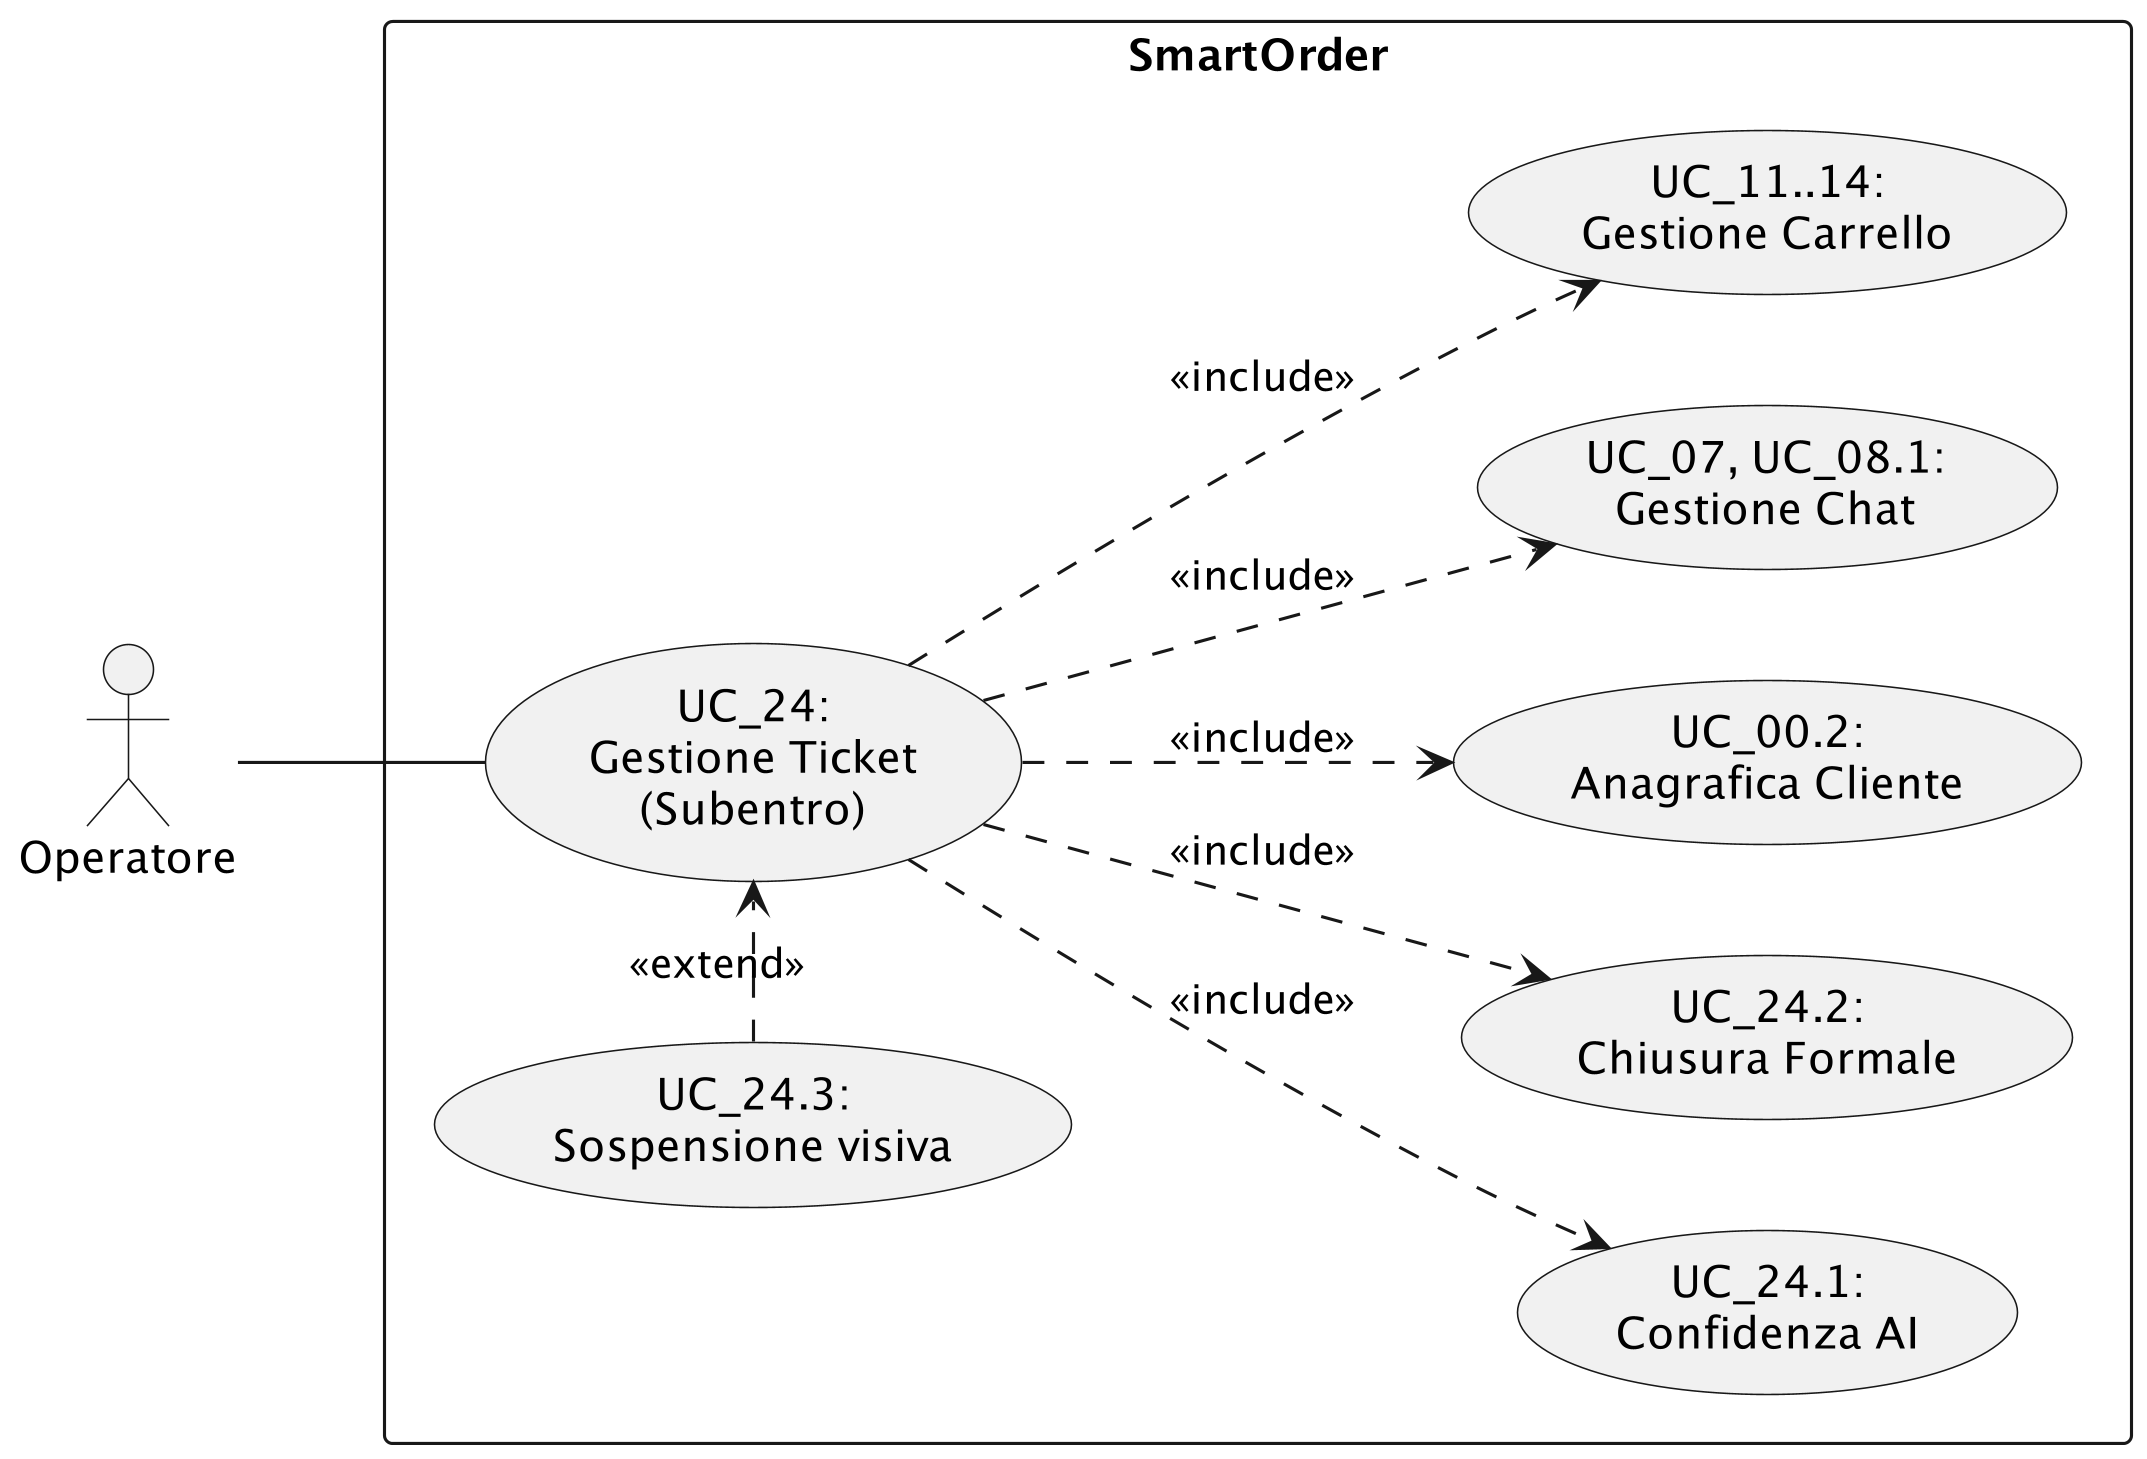
\includegraphics[width=0.8\textwidth]{uc-24.png}
    \caption{UC\_24: Gestione Ticket (Subentro Modale)}
\end{figure}

\begin{itemize}
    \item \textbf{Attore Principale}: Operatore
    \item \textbf{User Story}: Come Operatore, voglio avere a disposizione una console protetta in cui posso subentrare nella sessione di un Cliente per dirimere anomalie, comunicando con esso e manipolando i volumi del suo carrello da remoto.
    \item \textbf{Scenario Principale}: 
    \begin{enumerate}
        \item Il sistema intercetta l'apertura del ticket, registra l'assegnazione logica esclusiva (Lock) sull'Operatore ed espone la console in sovraimpressione (Modal).
        \item Il sistema inietta nell'intestazione le coordinate anagrafiche del Cliente $\rightarrow$ Include: \hyperref[uc_00.2]{UC\_00.2}
        \item Il sistema espone il flusso di comunicazione in tempo reale $\rightarrow$ Include: \hyperref[uc_07]{UC\_07}
        \item L'Operatore interagisce immettendo testo a supporto del Cliente $\rightarrow$ Include: \hyperref[uc_08.1]{UC\_08.1}
        \item L'Operatore manipola il carrello in delega (ricerca cataloghi, aggiunta logica, modifica quantità, rimozione) avvalendosi dei componenti standard di piattaforma $\rightarrow$ Include: \hyperref[uc_11]{UC\_11}, \hyperref[uc_12]{UC\_12}, \hyperref[uc_13]{UC\_13}, \hyperref[uc_14]{UC\_14}
        \item Contestualmente al carrello, esposizione del Livello di Confidenza AI $\rightarrow$ Vedi \hyperref[uc_24.1]{UC\_24.1}
        \item Chiusura formale della pratica $\rightarrow$ Vedi \hyperref[uc_24.2]{UC\_24.2}
    \end{enumerate}
    \item \textbf{Precondizioni}:
    \begin{itemize}
        \item L'Operatore si trova nella tabella "Ticket Aperti" e interagisce con un record in stato "Aperto" attualmente privo di Lock concorrente (nessun altro collega vi sta operando).
    \end{itemize}
    \item \textbf{Postcondizioni}:
    \begin{itemize}
        \item L'Operatore assume e mantiene il pieno controllo asincrono (Read/Write) sui dati di sessione del Cliente. Le variazioni applicate vengono salvate contestualmente nel DB del carrello remoto. Al termine, il Lock di sistema viene rilasciato.
    \end{itemize}
    \item \textbf{Inclusioni}:
    \begin{itemize}
        \item \hyperref[uc_00.2]{UC\_00.2}, \hyperref[uc_07]{UC\_07}, \hyperref[uc_08.1]{UC\_08.1}
        \item \hyperref[uc_11]{UC\_11}, \hyperref[uc_12]{UC\_12}, \hyperref[uc_13]{UC\_13}, \hyperref[uc_14]{UC\_14}
        \item \hyperref[uc_24.1]{UC\_24.1}, \hyperref[uc_24.2]{UC\_24.2}
    \end{itemize}
    \item \textbf{Estensioni}:
    \begin{itemize}
        \item Sospensione visiva temporanea dell'interfaccia $\rightarrow$ Vedi \hyperref[uc_24.3]{UC\_24.3}
    \end{itemize}
    \item \textbf{Trigger}: Selezione deliberata di un record interagibile dalla tabella di backoffice.
\end{itemize}

\subsubsection{UC\_24.1: Visualizzazione Livello di Confidenza AI}
\label{uc_24.1}
\begin{itemize}
    \item \textbf{Attore Principale}: Operatore
    \item \textbf{Scenario Principale}: A integrazione della visualizzazione standard del carrello (\hyperref[uc_13]{UC\_13}), il sistema espone contestualmente per ogni riga processata dall'Intelligenza Artificiale il relativo parametro di affidabilità (Confidence Score percentuale).
    \item \textbf{Postcondizioni}: L'Operatore dispone di una metrica tecnica e diagnostica, la cui visualizzazione resta rigorosamente invisibile ed esclusa dall'interfaccia pubblica del Cliente.
\end{itemize}

\subsubsection{UC\_24.2: Chiusura Formale Ticket}
\label{uc_24.2}
\begin{itemize}
    \item \textbf{Attore Principale}: Operatore
    \item \textbf{Scenario Principale}: L'Operatore innesca il comando di dismissione definitiva. Il database archivia lo stato in "Chiuso" ed esegue la revoca totale del token di Lock.
    \item \textbf{Postcondizioni}: Il sistema riabilita automaticamente le funzionalità di checkout sul terminale remoto del Cliente (comunicando il termine del subentro) e smonta l'istanza della console per l'Operatore.
\end{itemize}

\subsubsection{UC\_24.3: Sospensione visiva dell'interfaccia (Estensione)}
\label{uc_24.3}
\begin{itemize}
    \item \textbf{Attore Principale}: Operatore
    \item \textbf{Scenario Principale}: L'Operatore attiva il comando di chiusura contestuale (es. logica off-canvas o collasso visivo del layer modale). Il componente UI viene nascosto senza attuare procedure distruttive sui dati immessi.
    \item \textbf{Postcondizioni}: Il sistema mantiene rigorosamente inalterato lo stato "Aperto" del ticket e preserva il Lock di sicurezza sull'Operatore, permettendo a quest'ultimo l'ispezione protetta della dashboard sottostante o l'accesso ad altri moduli del gestionale per reperire informazioni.
\end{itemize}

% ==========================================
% GRUPPO H: GESTIONE STORICO ORDINI (OPERATORE)
% ==========================================

\subsection{UC\_25: Consultazione Storico Transazioni Globale}
\label{uc_25}

\begin{figure}[H]
    \centering 
    
\includegraphics[width=0.8\textwidth]{uc-25.png}
    \caption{UC\_25: Consultazione Storico Transazioni Globale}
\end{figure}

\begin{itemize}
    \item \textbf{Attore Principale}: Operatore
    \item \textbf{User Story}: Come Operatore, voglio poter visualizzare una vista riepilogativa contenente lo storico globale delle transazioni effettuate da tutti i clienti, affinché io possa monitorare e controllare il flusso degli ordini ricevuti in piattaforma.
    \item \textbf{Scenario Principale}: 
    \begin{enumerate}
        \item Il sistema interroga il database locale della webapp e struttura l'elenco dei record transazionali.
        \item Il sistema applica un ordinamento logico predefinito (discendente basato sulla data di transazione), evidenziando il criterio attivo tramite apposito indicatore grafico.
        \item Per ogni transazione, esposizione delle coordinate temporali e di sistema $\rightarrow$ Include: \hyperref[uc_00.3]{UC\_00.3}
        \item Per ogni transazione, esposizione dell'anagrafica aziendale associata $\rightarrow$ Include: \hyperref[uc_00.2]{UC\_00.2}
    \end{enumerate}
    \item \textbf{Precondizioni}:
    \begin{itemize}
        \item L'Operatore ha richiesto l'accesso alla dashboard di competenza (tramite \hyperref[uc_19.2]{UC\_19.2}).
    \end{itemize}
    \item \textbf{Postcondizioni}:
    \begin{itemize}
        \item L'interfaccia espone l'elenco delle transazioni, permettendo all'Operatore di utilizzare i controlli di ricerca o di selezionare un record per ispezionarne i dettagli completi.
    \end{itemize}
    \item \textbf{Inclusioni}:
    \begin{itemize}
        \item \hyperref[uc_00.2]{UC\_00.2}, \hyperref[uc_00.3]{UC\_00.3}
    \end{itemize}
    \item \textbf{Estensioni}:
    \begin{itemize}
        \item Inversione dell'ordinamento cronologico $\rightarrow$ Vedi \hyperref[uc_25.1]{UC\_25.1}
        \item Ricezione aggiornamento asincrono (Live Sync) $\rightarrow$ Vedi \hyperref[uc_25.2]{UC\_25.2}
        \item Filtraggio Temporale dei Record $\rightarrow$ Extend: \hyperref[uc_20]{UC\_20}
        \item Ricerca Mirata a Colonna Singola $\rightarrow$ Extend: \hyperref[uc_21]{UC\_21}
    \end{itemize}
\end{itemize}

\subsubsection{UC\_25.1: Ordinamento dinamico della colonna}
\label{uc_25.1}
\begin{itemize}
    \item \textbf{Attore Principale}: Operatore
    \item \textbf{Scenario Principale}: L'Operatore innesca il comando di ordinamento interagendo con le intestazioni. Il sistema riposiziona la priorità dell'array di visualizzazione (da ascendente a discendente o viceversa) aggiornando la freccia direzionale.
\end{itemize}

\subsubsection{UC\_25.2: Ricezione aggiornamento in tempo reale (Live Sync)}
\label{uc_25.2}
\begin{itemize}
    \item \textbf{Attore Principale}: Operatore
    \item \textbf{Scenario Principale}: L'interfaccia capta l'evento di un nuovo checkout concluso tramite socket web. Il sistema esegue l'iniezione silente del nuovo record in cima all'elenco, rispettando l'ordine imposto senza forzare ricaricamenti pagina.
\end{itemize}


% -------------------------------------------------------------------

\subsection{UC\_26: Ispezione Dettaglio Ordine Globale}
\label{uc_26}

\begin{figure}[H]
    \centering 
    
\includegraphics[width=0.8\textwidth]{uc-26.png}
    \caption{UC\_26: Ispezione Dettaglio Ordine Globale}
\end{figure}

\begin{itemize}
    \item \textbf{Attore Principale}: Operatore
    \item \textbf{User Story}: Come Operatore, voglio aprire una scheda approfondita dell'ordine per ispezionarne il contenuto logistico e il contesto conversazionale originario.
    \item \textbf{Scenario Principale}: 
    \begin{enumerate}
        \item Il sistema istanzia l'interfaccia dedicata ai dettagli dell'ordine in sovraimpressione (Modal).
        \item Esposizione coordinate generali e anagrafica Cliente $\rightarrow$ Include: \hyperref[uc_00.2]{UC\_00.2}, \hyperref[uc_00.3]{UC\_00.3}
        \item Esposizione log conversazionale storico $\rightarrow$ Include: \hyperref[uc_00.4]{UC\_00.4}
        \item Per ogni riga d'ordine, esposizione dei metadati prodotto $\rightarrow$ Include: \hyperref[uc_00.1]{UC\_00.1}
        \item Per ogni riga d'ordine, esposizione della quantità definitiva $\rightarrow$ Include: \hyperref[uc_17.1]{UC\_17.1}
        \item Esposizione Livello Confidenza AI $\rightarrow$ Vedi \hyperref[uc_26.1]{UC\_26.1}
    \end{enumerate}
    \item \textbf{Precondizioni}:
    \begin{itemize}
        \item La tabella "Ordini" (\hyperref[uc_25]{UC\_25}) è attiva e l'Operatore ha interagito con un record valido.
    \end{itemize}
    \item \textbf{Postcondizioni}:
    \begin{itemize}
        \item Il sistema espone il dettaglio completo dell'ordine e il log conversazionale in modalità puramente consultiva, garantendo l'assoluta immutabilità dello storico. Si ribadisce l'assenza di dati legati al pricing, delegati all'ERP esterno.
    \end{itemize}
    \item \textbf{Inclusioni}:
    \begin{itemize}
        \item \hyperref[uc_00.1]{UC\_00.1}, \hyperref[uc_00.2]{UC\_00.2}, \hyperref[uc_00.3]{UC\_00.3}, \hyperref[uc_00.4]{UC\_00.4}, \hyperref[uc_17.1]{UC\_17.1}, \hyperref[uc_26.1]{UC\_26.1}
    \end{itemize}
    \item \textbf{Estensioni}:
    \begin{itemize}
        \item Sospensione dell'ispezione visiva $\rightarrow$ Vedi \hyperref[uc_26.2]{UC\_26.2}
    \end{itemize}
    \item \textbf{Trigger}: L'Operatore attiva il comando di ispezione espandendo un record specifico della tabella.
\end{itemize}

\subsubsection{UC\_26.1: Visualizzazione Livello di Confidenza AI}
\label{uc_26.1}
\begin{itemize}
    \item \textbf{Attore Principale}: Operatore
    \item \textbf{Scenario Principale}: A corredo della riga prodotto, il sistema preleva il metadato valutativo originato dall'LLM al momento dell'interpretazione semantica e lo esplicita graficamente per consentire all'Operatore verifiche diagnostiche sull'algoritmo.
\end{itemize}

\subsubsection{UC\_26.2: Sospensione dell'ispezione}
\label{uc_26.2}
\begin{itemize}
    \item \textbf{Attore Principale}: Operatore
    \item \textbf{Scenario Principale}: L'Operatore innesca il comando di chiusura contestuale.
    \item \textbf{Postcondizioni}: Il sistema smonta l'istanza grafica di dettaglio e ripristina il focus primario sulla vista tabellare principale.
\end{itemize}

% ==========================================
% GRUPPO I: OTTIMIZZAZIONE AI (HUMAN-IN-THE-LOOP)
% ==========================================

\subsection{UC\_27: Consultazione Log e Discrepanze AI}
\label{uc_27}

\begin{figure}[H]
    \centering 
    
\includegraphics[width=0.8\textwidth]{uc-27.png}
    \caption{UC\_27: Consultazione Log e Discrepanze AI}
\end{figure}

\begin{itemize}
    \item \textbf{Attore Principale}: Operatore
    \item \textbf{User Story}: Come Operatore, voglio consultare i record dei feedback negativi o delle correzioni manuali ai carrelli, affinché io possa supervisionare il comportamento dell'AI e alimentare il suo dataset di addestramento (Retraining\textsubscript{\textsc{g}}).
    \item \textbf{Scenario Principale}: 
    \begin{enumerate}
        \item Il sistema recupera i dati dai log di telemetria semantica immagazzinati nel database.
        \item Il sistema applica un ordinamento logico predefinito (discendente basato sul timestamp), evidenziando il criterio attivo tramite apposito indicatore grafico.
        \item Esposizione testuale dell'Input originario $\rightarrow$ Vedi \hyperref[uc_27.1]{UC\_27.1}
        \item Esposizione della Risposta LLM $\rightarrow$ Vedi \hyperref[uc_27.2]{UC\_27.2}
        \item Esposizione della Classificazione Utente $\rightarrow$ Vedi \hyperref[uc_27.3]{UC\_27.3}
        \item Esposizione della Correzione (Delta) $\rightarrow$ Vedi \hyperref[uc_27.4]{UC\_27.4}
        \item Esposizione dei Controlli di Azione $\rightarrow$ Vedi \hyperref[uc_27.5]{UC\_27.5}
        \item Esposizione del Timestamp di sistema $\rightarrow$ Vedi \hyperref[uc_27.6]{UC\_27.6}
    \end{enumerate}
    \item \textbf{Precondizioni}:
    \begin{itemize}
        \item L'Operatore ha richiesto l'accesso al modulo "Ottimizzazione AI" (\hyperref[uc_19.3]{UC\_19.3}).
    \end{itemize}
    \item \textbf{Postcondizioni}:
    \begin{itemize}
        \item Il sistema applica un filtro logico nativo omettendo i record già processati e mostrando di default unicamente i nodi in stato "Da gestire".
    \end{itemize}
    \item \textbf{Inclusioni}:
    \begin{itemize}
        \item \hyperref[uc_27.1]{UC\_27.1}, \hyperref[uc_27.2]{UC\_27.2}, \hyperref[uc_27.3]{UC\_27.3}, \hyperref[uc_27.4]{UC\_27.4}, \hyperref[uc_27.5]{UC\_27.5}, \hyperref[uc_27.6]{UC\_27.6}
    \end{itemize}
    \item \textbf{Estensioni}:
    \begin{itemize}
        \item Ordinamento dinamico della colonna $\rightarrow$ Vedi \hyperref[uc_27.7]{UC\_27.7}
        \item Propagazione socket di sistema (Live Sync) $\rightarrow$ Vedi \hyperref[uc_27.8]{UC\_27.8}
        \item Filtraggio Temporale dei Record $\rightarrow$ Extend: \hyperref[uc_20]{UC\_20}
        \item Esecuzione Ricerca Globale Multi-Campo $\rightarrow$ Extend: \hyperref[uc_22]{UC\_22}
        \item Filtraggio Segnalazioni per Stato $\rightarrow$ Extend: \hyperref[uc_28]{UC\_28}
    \end{itemize}
\end{itemize}

\subsubsection{UC\_27.1: Esposizione Input originario}
\label{uc_27.1}
\begin{itemize}
    \item \textbf{Attore Principale}: Operatore
    \item \textbf{Scenario Principale}: Il sistema estrae e rende consultabile la trascrizione testuale esatta derivata dalla sorgente utente (audio o testo) che ha scatenato l'inferenza.
\end{itemize}

\subsubsection{UC\_27.2: Esposizione Risposta LLM}
\label{uc_27.2}
\begin{itemize}
    \item \textbf{Attore Principale}: Operatore
    \item \textbf{Scenario Principale}: Il sistema renderizza il tracciato di output logico originato dal bot durante la conversazione.
\end{itemize}

\subsubsection{UC\_27.3: Esposizione Classificazione Utente}
\label{uc_27.3}
\begin{itemize}
    \item \textbf{Attore Principale}: Operatore
    \item \textbf{Scenario Principale}: Il sistema espone in un layout a tag la macro-categoria dell'errore, le opzioni selezionate ed eventuali note esplicative fornite dal Cliente al momento del feedback negativo (\hyperref[uc_09.2]{UC\_09.2}).
\end{itemize}

\subsubsection{UC\_27.4: Esposizione Correzione Rilevata (Delta)}
\label{uc_27.4}
\begin{itemize}
    \item \textbf{Attore Principale}: Operatore
    \item \textbf{Scenario Principale}: Il sistema calcola e formatta in modo compatto le deviazioni riscontrate tra il carrello suggerito in origine dall'AI e l'elaborazione correttiva finale eseguita in modo manuale (es. identificando l'azione "+1 Acqua, -1 Birra").
\end{itemize}

\subsubsection{UC\_27.5: Esposizione Controlli di Azione}
\label{uc_27.5}
\begin{itemize}
    \item \textbf{Attore Principale}: Operatore
    \item \textbf{Scenario Principale}: Il sistema istanzia dinamicamente i comandi logici interagibili sulla base dello stato di validazione attuale del record (Approvazione, Rigetto, Revoca).
\end{itemize}

\subsubsection{UC\_27.6: Esposizione Timestamp}
\label{uc_27.6}
\begin{itemize}
    \item \textbf{Attore Principale}: Operatore
    \item \textbf{Scenario Principale}: Il sistema stampa il marcatore temporale (data e ora) di innesco del log.
\end{itemize}

\subsubsection{UC\_27.7: Ordinamento dinamico della colonna}
\label{uc_27.7}
\begin{itemize}
    \item \textbf{Attore Principale}: Operatore
    \item \textbf{Scenario Principale}: L'Operatore innesca il controllo d'ordinamento. L'array di dati muta la propria disposizione (ascendente/discendente) in ottemperanza al comando richiesto.
\end{itemize}

\subsubsection{UC\_27.8: Ricezione aggiornamenti in tempo reale (Live Sync)}
\label{uc_27.8}
\begin{itemize}
    \item \textbf{Attore Principale}: Operatore
    \item \textbf{Scenario Principale}: Il socket capta un evento remoto di telemetria. Il sistema provvede all'innesto asincrono della nuova segnalazione in testa all'interfaccia, preservando la coerenza operativa del backoffice.
\end{itemize}

% -------------------------------------------------------------------

\subsection{UC\_29: Ispezione Contesto Segnalazione}
\label{uc_29}

\begin{figure}[H]
    \centering 
    
\includegraphics[width=0.8\textwidth]{uc-29.png}
    \caption{UC\_29: Ispezione Contesto Segnalazione}
\end{figure}

\begin{itemize}
    \item \textbf{Attore Principale}: Operatore
    \item \textbf{User Story}: Come Operatore, voglio poter leggere la chat originale tra il Cliente e l'AI associata a una specifica segnalazione, affinché io possa disambiguare il contesto dell'errore prima di valutarlo.
    \item \textbf{Scenario Principale}: 
    \begin{enumerate}
        \item A seguito dell'attivazione logica dell'espansione del record, il sistema istanzia una finestra protetta in sovraimpressione.
        \item Il sistema attinge al Session ID e assembla il tracciato storico di comunicazione $\rightarrow$ Include: \hyperref[uc_00.4]{UC\_00.4}
    \end{enumerate}
    \item \textbf{Precondizioni}:
    \begin{itemize}
        \item L'Operatore si trova nella dashboard "Ottimizzazione AI" (\hyperref[uc_27]{UC\_27}) e interagisce con un record specifico.
    \end{itemize}
    \item \textbf{Postcondizioni}:
    \begin{itemize}
        \item L'Operatore dischiude gli elementi di contesto indispensabili alla formulazione di un verdetto sull'anomalia, operando in una logica di sola lettura.
    \end{itemize}
    \item \textbf{Inclusioni}:
    \begin{itemize}
        \item \hyperref[uc_00.4]{UC\_00.4}
    \end{itemize}
    \item \textbf{Trigger}: Interazione sul comando d'estensione (es. click di riga) della singola segnalazione.
\end{itemize}

% -------------------------------------------------------------------

\subsection{UC\_30: Validazione Segnalazione "Da Gestire"}
\label{uc_30}

\begin{figure}[H]
    \centering 
    
\includegraphics[width=0.8\textwidth]{uc-30.png}
    \caption{UC\_30: Validazione Segnalazione "Da Gestire"}
\end{figure}

\begin{itemize}
    \item \textbf{Attore Principale}: Operatore
    \item \textbf{User Story}: Come Operatore, voglio poter definire lo stato di un'anomalia AI valutando se essa rappresenti effettivamente un errore algoritmico utile all'addestramento (Approvazione) o un falso allarme (Scarto).
    \item \textbf{Scenario Principale}: 
    \begin{enumerate}
        \item L'Operatore formula e trasmette la risoluzione di merito sull'istanza analizzata avvalendosi dei comandi di riga.
        \item Assegnazione attributo logico positivo $\rightarrow$ Vedi \hyperref[uc_30.1]{UC\_30.1}
        \item Assegnazione attributo logico negativo $\rightarrow$ Vedi \hyperref[uc_30.2]{UC\_30.2}
    \end{enumerate}
    \item \textbf{Precondizioni}:
    \begin{itemize}
        \item Il record log in fase di ispezione si trova rigorosamente nello stato "Da gestire".
    \end{itemize}
    \item \textbf{Inclusioni}:
    \begin{itemize}
        \item \hyperref[uc_30.1]{UC\_30.1}, \hyperref[uc_30.2]{UC\_30.2}
    \end{itemize}
    \item \textbf{Trigger}: Volontà dell'Operatore di prendere in carico e smarcare definitivamente una segnalazione pendente.
\end{itemize}

\subsubsection{UC\_30.1: Approvazione Segnalazione}
\label{uc_30.1}
\begin{itemize}
    \item \textbf{Attore Principale}: Operatore
    \item \textbf{Scenario Principale}: L'Operatore immette l'ordine di validazione positiva.
    \item \textbf{Postcondizioni}: Il sistema promuove la risorsa logica convertendone lo stato interno in "Accettata". I payload informativi (Input e Delta di correzione) vengono predisposti e rilasciati all'infrastruttura AI per le fasi di apprendimento continuo (Retraining).
    \item \textbf{Trigger}: Comando logico di approvazione.
\end{itemize}

\subsubsection{UC\_30.2: Scarto Segnalazione}
\label{uc_30.2}
\begin{itemize}
    \item \textbf{Attore Principale}: Operatore
    \item \textbf{Scenario Principale}: L'Operatore immette l'ordine di nullità, giudicando la segnalazione come falso positivo o errore umano imputabile al Cliente.
    \item \textbf{Postcondizioni}: Il sistema destituisce l'entità degradandola a "Rifiutata". L'integrazione ai fini dell'apprendimento abortisce in via definitiva e l'informazione viene scartata dalle pipeline dell'amministrazione AI.
    \item \textbf{Trigger}: Comando logico di scarto o rigetto.
\end{itemize}

% -------------------------------------------------------------------

\subsection{UC\_31: Revoca Segnalazione "Accettata"}
\label{uc_31}

\begin{figure}[H]
    \centering 
    
\includegraphics[width=0.6\textwidth]{uc-31.png}
    \caption{UC\_31: Revoca Segnalazione "Accettata"}
\end{figure}

\begin{itemize}
    \item \textbf{Attore Principale}: Operatore
    \item \textbf{User Story}: Come Operatore, voglio poter annullare una validazione positiva elargita per errore, al fine di evitare la contaminazione ("avvelenamento") del dataset di addestramento dell'AI.
    \item \textbf{Scenario Principale}: 
    \begin{enumerate}
        \item L'Operatore emette una direttiva di ripristino (Rollback) interagendo con l'apposito controllo di riga.
    \end{enumerate}
    \item \textbf{Precondizioni}:
    \begin{itemize}
        \item La dashboard sta attualmente esponendo le entità filtrate in base all'attributo "Accettate" (tramite \hyperref[uc_28]{UC\_28}).
    \end{itemize}
    \item \textbf{Postcondizioni}:
    \begin{itemize}
        \item Il sistema attua l'inversione logica, declassando il record allo stato originario "Da gestire". I dati vengono invalidati e rimossi dal repository di elaborazione del Retraining, venendo reinseriti forzatamente nella coda di esame standard per una nuova valutazione.
    \end{itemize}
    \item \textbf{Trigger}: Attivazione del comando d'inversione logica (Undo).
\end{itemize}